% !TEX program = xelatex
% =============================================================================
% Block Round --- 수업 지도안 (ko-KR)
% 대한민국 고등학교 3학년 (고3)을 위한 5차시 수업 시퀀스, 마인크래프트 우주 정박.
% Estilo grafico alinhado a docs_math/Block_Round_Math_ko-KR.pdf
% Compilacao: xelatex Plano_de_Aula_ko-KR.tex  (executar duas vezes p/ TOC + refs)
% =============================================================================
\documentclass[12pt,a4paper]{scrartcl}

% ---------- Idioma e fontes (Coreano via xeCJK + Malgun Gothic) ---------------
\usepackage{fontspec}
\usepackage{xeCJK}
\xeCJKsetup{CJKspace=true}
\XeTeXlinebreaklocale "ko"
\XeTeXlinebreakskip=0pt plus 1pt minus 0.1pt
\setCJKmainfont{Malgun Gothic}[Scale=1.05]
\setCJKsansfont{Malgun Gothic}[Scale=1.05]
\setmainfont{Latin Modern Roman}[Scale=1.05]
\setsansfont{Latin Modern Sans}[Scale=1.05]
\setmonofont{Latin Modern Mono}
\usepackage{unicode-math}
\setmathfont{Latin Modern Math}[Scale=1.05]

% ---------- Pacotes ----------------------------------------------------------
\usepackage{amsmath}
\usepackage{mathtools}

\usepackage[a4paper,top=2.8cm,bottom=2.8cm,left=2.6cm,right=2.6cm,
            headheight=16pt]{geometry}
\usepackage{microtype}
\usepackage{xcolor}
\usepackage{booktabs}
\usepackage{array}
\usepackage{tabularx}
\usepackage{enumitem}
\usepackage{titlesec}
\usepackage{fancyhdr}
\usepackage{graphicx}
\usepackage{csquotes}
\usepackage{tcolorbox}
\tcbuselibrary{skins,breakable}
\usepackage{needspace}
\usepackage{caption}
\usepackage{subcaption}
\usepackage{float}

\raggedbottom

% ---------- Paleta cromatica Block Round -------------------------------------
\definecolor{accent}{HTML}{5B8E3F}      % verde-grama Minecraft
\definecolor{accentdark}{HTML}{406A2A}
\definecolor{earth}{HTML}{825432}        % marrom-dirt
\definecolor{ink}{HTML}{1F1F23}
\definecolor{muted}{HTML}{4E4E58}
\definecolor{bg}{HTML}{FBF6E9}
\definecolor{rule}{HTML}{D8D1BC}
\definecolor{linkc}{HTML}{2D5A1F}

\usepackage[colorlinks=true,
            linkcolor=linkc,
            urlcolor=linkc,
            citecolor=linkc,
            breaklinks=true,
            bookmarks=true,bookmarksopen=true,
            pdftitle={Block Round --- 수업 지도안 (ko-KR)},
            pdfauthor={Vinicius Rodrigues de Souza}]{hyperref}
\usepackage{xurl}

\color{ink}

\widowpenalty=10000
\clubpenalty=10000

% ---------- Estilo de secoes -------------------------------------------------
\titleformat{\section}
  {\sffamily\Large\bfseries\color{accent}}{\thesection.}{0.6em}{}
\titleformat{\subsection}
  {\sffamily\large\bfseries\color{accent!85!ink}}{\thesubsection}{0.6em}{}
\titleformat{\subsubsection}
  {\sffamily\normalsize\bfseries\color{muted}}{\thesubsubsection}{0.5em}{}
\titlespacing*{\section}{0pt}{1.2\baselineskip}{0.6\baselineskip}
\titlespacing*{\subsection}{0pt}{0.8\baselineskip}{0.3\baselineskip}
\titlespacing*{\subsubsection}{0pt}{0.6\baselineskip}{0.2\baselineskip}

% ---------- Cabecalho e rodape -----------------------------------------------
\pagestyle{fancy}
\fancyhf{}
\fancyhead[L]{\small\sffamily\bfseries\color{accent}BLOCK ROUND}
\fancyhead[R]{\small\sffamily\color{muted}수업 지도안 --- 고등학교 3학년}
\fancyfoot[L]{\small\sffamily\color{muted}Block Round --- 교수학습 자료}
\fancyfoot[R]{\small\sffamily\color{muted}\thepage 페이지}
\renewcommand{\headrulewidth}{0.4pt}
\renewcommand{\footrulewidth}{0.4pt}
\renewcommand{\headrule}{{\color{rule}\hrule height \headrulewidth}}
\renewcommand{\footrule}{{\color{rule}\vskip-\footrulewidth\hrule height \footrulewidth\vskip-\footrulewidth}}

% ---------- Caixas didaticas -------------------------------------------------
\newtcolorbox{susik}{
  colback=bg, colframe=rule, boxrule=0.4pt, arc=2pt,
  left=10pt,right=10pt,top=8pt,bottom=8pt,
  before skip=8pt, after skip=8pt,
  fontupper=\color{accentdark}, breakable,
  before={\par\needspace{4\baselineskip}}
}

\newtcolorbox{hwaldong}[1][활동]{
  enhanced, breakable,
  colback=bg, colframe=accent, boxrule=0.6pt, arc=4pt,
  left=12pt,right=12pt,top=10pt,bottom=10pt,
  before skip=12pt, after skip=12pt,
  before={\par\needspace{5\baselineskip}},
  attach boxed title to top left={xshift=10pt,yshift=-8pt},
  boxed title style={colback=accent,colframe=accent,boxrule=0pt,arc=2pt},
  coltitle=white, fonttitle=\sffamily\bfseries\small,
  title=#1
}

\newtcolorbox{memo}[1][지도상의 유의점]{
  enhanced, breakable,
  colback=bg!50!white, colframe=rule, boxrule=0.4pt, arc=2pt,
  left=10pt,right=10pt,top=8pt,bottom=8pt,
  before skip=8pt, after skip=8pt,
  before={\par\needspace{3\baselineskip}},
  attach boxed title to top left={xshift=10pt,yshift=-7pt},
  boxed title style={colback=muted,colframe=muted,boxrule=0pt,arc=2pt},
  coltitle=white, fonttitle=\sffamily\bfseries\footnotesize,
  title=#1
}

\newtcolorbox{pyojun}[1][교육과정]{
  enhanced,
  breakable=false,
  colback=bg!70!white, colframe=accent!60!ink, boxrule=0.4pt, arc=2pt,
  left=10pt,right=10pt,top=6pt,bottom=6pt,
  before skip=6pt, after skip=6pt,
  before={\par\needspace{8\baselineskip}},
  attach boxed title to top left={xshift=10pt,yshift=-6pt},
  boxed title style={colback=accent!60!ink,colframe=accent!60!ink,boxrule=0pt,arc=2pt},
  coltitle=white, fonttitle=\sffamily\bfseries\footnotesize,
  title=#1
}

\newtcolorbox{minecraft}[1][마인크래프트]{
  enhanced, breakable,
  colback=accent!7, colframe=earth!70!accent, boxrule=0.5pt, arc=3pt,
  left=10pt,right=10pt,top=8pt,bottom=8pt,
  before skip=10pt, after skip=10pt,
  before={\par\needspace{3\baselineskip}},
  attach boxed title to top left={xshift=10pt,yshift=-7pt},
  boxed title style={colback=earth,colframe=earth,boxrule=0pt,arc=2pt},
  coltitle=white, fonttitle=\sffamily\bfseries\footnotesize,
  title=#1
}

\setlength{\parskip}{0.75em}
\setlength{\parindent}{0pt}
\linespread{1.10}

\setlength{\textfloatsep}{14pt plus 2pt minus 2pt}
\setlength{\floatsep}{14pt plus 2pt minus 2pt}
\setlength{\intextsep}{14pt plus 2pt minus 2pt}

\captionsetup{font=small, labelfont={bf,color=accent}, textfont={color=muted}, justification=centering}
\captionsetup[sub]{font=footnotesize, labelfont={bf,color=accent!75!ink}, textfont={color=muted}}

\graphicspath{{img/}}

\newcommand{\code}[1]{\texttt{\small #1}}
\newcommand{\acc}[1]{\textcolor{accent}{\textbf{#1}}}
\newcommand{\cmd}[1]{\textcolor{earth}{\texttt{\small #1}}}
\newcommand{\tempo}[1]{\textnormal{\footnotesize\color{bg!90!white}\textsf{#1}}}

\begin{document}

% =============================================================================
% 표지
% =============================================================================
\begin{titlepage}
  \centering
  \vspace*{3.0cm}
  {\sffamily\bfseries\fontsize{56}{60}\selectfont \color{accent} Block Round\par}
  \vspace{0.7cm}
  {\sffamily\LARGE\color{muted} 수업 지도안\par}
  \vspace{0.25cm}
  {\sffamily\Large\color{muted} 고등학교 3학년 (고3)\par}
  \vspace{1.0cm}
  {\color{rule}\rule{0.6\textwidth}{0.6pt}\par}
  \vspace{0.7cm}
  \begin{minipage}{0.84\textwidth}
    \centering\color{ink}\large
    대한민국 고등학교 3학년 학생들에게 \emph{Block Round} 생성기를 소개하는
    5차시 수업 시퀀스입니다. \emph{기하} (해석기하), \emph{컴퓨팅 사고},
    \emph{디지털 리터러시}, 그리고 \emph{마인크래프트 게임 안에서의 건축}을
    하나의 문제 주위로 결합합니다: 어떻게 연속 곡면을 유한한 복셀 격자
    위에 표현하고, 그 표현을 우리나라 청소년들에게 가장 친숙한 디지털 우주
    안에서 건축 가능한 구조로 옮길 것인가?
  \end{minipage}
  \vspace{0.7cm}\\
  {\color{rule}\rule{0.6\textwidth}{0.6pt}\par}
  \vspace{0.9cm}
  \begin{minipage}{0.78\textwidth}
    \centering
    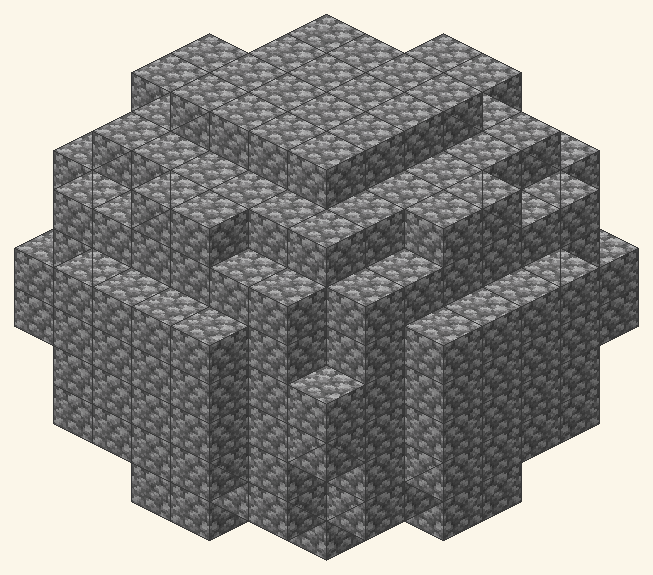
\includegraphics[width=0.55\linewidth]{fig10_3d_sphere_d12.png}\\[0.4em]
    {\sffamily\footnotesize\color{muted}Block Round로 복셀화된 지름 10의 구로,
    마인크래프트의 \emph{cobblestone} (둥근돌) 텍스처로 렌더링하였습니다.}
  \end{minipage}
  \vspace{0.7cm}\\
  {\color{rule}\rule{0.6\textwidth}{0.6pt}\par}
  \vspace{0.9cm}
  \begin{minipage}{0.82\textwidth}
    \centering\sffamily\small\color{muted}
    \textbf{통합 영역:} 수학 $\cdot$ 국어 (디지털 예술, 디자인) $\cdot$ 정보 $\cdot$ 디지털 리터러시 $\cdot$ 게임 교육 \\[0.4em]
    \textbf{정렬:} 2022 개정 교육과정 --- 고등학교 $\cdot$ 「기하」, 「미적분 II」, 「대수」 $\cdot$ 대학수학능력시험 (수능) $\cdot$ \hyperref[sec:olympiad]{KMO/KOI} $\cdot$ 마인크래프트 에듀케이션
  \end{minipage}
\end{titlepage}

% =============================================================================
\renewcommand{\contentsname}{\color{accent}목차}
\tableofcontents
\thispagestyle{fancy}
\newpage

% =============================================================================
\section{개관과 맥락}\label{sec:identificacao}

\begin{center}
\begin{tabular}{@{}p{0.32\textwidth}p{0.62\textwidth}@{}}
\toprule
\textbf{교과목} & 수학 (예술, 정보, 공학, 역사, 지리와의 강한 학제간 연계). \\
\addlinespace[2pt]
\textbf{학교급과 학년} & 고등학교 3학년 (고3, 일반고등학교 / 자율형 사립고 / 외국어고 / 과학고 / 특성화고 등). 2학년과 방송통신고등학교 (방통고)에도 적용 가능. \\
\addlinespace[2pt]
\textbf{대상 학교 유형} & 주간 일반고, 야간 일반고, 방송통신고, 진로집중과정, 산업수요맞춤형고 (마이스터고 및 특성화고 통합과정) 통합형 직업교육. \\
\addlinespace[2pt]
\textbf{수업 시수} & 50분 5차시 (수업 250분) + 선택적 과외 활동. 100분 블록 시간표 변형은 §\ref{sec:adapt}에서 설명. \\
\addlinespace[2pt]
\textbf{핵심 자원} & Block Round --- 무료 \emph{웹} 애플리케이션, 가입 불필요, 서버 없음, 브라우저에서 오프라인 실행 (PWA). 「개인정보 보호법」 (PIPA) 준수: 개인정보 수집·전송하지 않음. 저가 \emph{스마트폰}에서도 실행 가능 --- 자바 불필요, 마인크래프트 설치 불필요. \\
\addlinespace[2pt]
\textbf{2022 개정 교육과정 영역} & 「기하」 (원, 타원, 쌍곡선, 포물선, 공간도형) $\cdot$ 「미적분 II」 (적분과 입체도형의 부피) $\cdot$ 「대수」 (벡터 옵션) $\cdot$ 「정보과」 (인공지능 수학 연계). \\
\addlinespace[2pt]
\textbf{선택과목 연결} & 일반선택: 대수, 미적분 I/II, 확률과 통계, 기하. 진로선택: 인공지능 수학, 직무 수학, 경제 수학. 융합선택: 수학과제 탐구, 실용 통계, 수학과 문화. 학생부 종합 전형의 탐구 활동에도 적합. \\
\addlinespace[2pt]
\textbf{연계 활동} & \hyperref[sec:olympiad]{한국수학올림피아드 (KMO --- 대한수학회)} $\cdot$ 한국정보올림피아드 (KOI) $\cdot$ 과학전람회 $\cdot$ 자유학기제 (중3 적용 가능) $\cdot$ 마인크래프트 에듀케이션 에디션 (한국 마이크로소프트 + 교육부 협력). \\
\addlinespace[2pt]
\textbf{선수 학습} & 좌표평면; 원의 방정식 (고1 「공통수학2」); 입체도형의 부피와 표면적 (중3·고2); 함수의 개념; 비례와 백분율. \emph{마인크래프트} 사용 경험 (권장하나 필수 아님; \emph{Block Round} 소프트웨어 자체는 게임 없이 작동). \\
\addlinespace[2pt]
\textbf{교사 사전 준비} & Block Round 사전 탐구 20분; \texttt{docs\_math/Block\_Round\_Math\_ko-KR.pdf} (한국어 기술 문서) 읽기; 선택적으로 마인크래프트 자바 에디션의 \cmd{/fill}, \cmd{/clone}, \cmd{//sphere} 명령어 표면적 접촉. \\
\bottomrule
\end{tabular}
\end{center}

\begin{memo}[대한민국 고등학교의 다양성]
이 시퀀스는 한국 고등학교 교육의 다층적 맥락을 위해 설계되었습니다: 서울/부산/인천/광주/대구/대전 등 수도권과 광역시의 일반고; 외국어고, 과학고 같은 특수목적고 (특목고); 마이스터고와 특성화고; 자율형 사립고 (자사고); 강원·전남·제주 등 농산어촌·도서벽지의 작은 학교; 다문화 학생 비율이 높은 안산·시흥·화성 지역의 학교; 방송통신고와 평생교육 시설. 각 맥락마다 §\ref{sec:adapt}에서 구체적인 조정안을 제시합니다. Block Round가 선택된 이유는 \emph{이 모든 환경에 작동하기 때문입니다}: 저가 \emph{스마트폰}에서 실행되고, 첫 로딩 이후 인터넷이 필요 없으며 (PWA), 가입이나 주민등록번호도 요구하지 않고, 「개인정보 보호법」 (PIPA, 2011년 시행, 2023년 개정)의 요건에 따라 개인정보를 수집하지 않습니다.
\end{memo}

\begin{minecraft}[왜 마인크래프트를 매개로 삼는가]
마인크래프트는 역사상 가장 많이 팔린 비디오 게임입니다 (3억 부 이상). 한국에서는 2014년 무렵부터 청소년 사이에 강한 영향력을 행사하며, 양띵·우왁굳·풍월량·침착맨 같은 유명 스트리머들이 마인크래프트 콘텐츠를 통해 청소년 문화에 큰 발자국을 남겼습니다. \emph{샌드박스 네트워크}와 같은 한국 콘텐츠 제작사는 마인크래프트 교육 영상의 매니지먼트를 담당하고 있습니다. 한국정보화진흥원 (NIA)의 「청소년 인터넷 이용실태조사」와 통계청 자료에 의하면 마인크래프트는 지속적으로 한국 10대 청소년이 가장 많이 즐기는 게임 중 하나로 나타납니다. \emph{마인크래프트를 모티프로 삼는 것은 유행 따라가기가 아닙니다. 한국 청소년이 이미 살고 있고, 이미 기하를 실천하는 공간을 인정하는 것입니다.}
\end{minecraft}

% =============================================================================
\section{교육적 정당화}\label{sec:justificativa}

대한민국 고3 수학 수업에서 Block Round를 교수학습 도구로 선택한 이유는 한국 현대 교육의 \acc{다섯 가지} 요구에 부합하기 때문입니다: 형식적 수학과 디지털 문화의 통합 (2022 개정 교육과정 「디지털 새싹 교실」 정책); 추상적 지식을 학생에게 \emph{의미 있는} 실천으로 맥락화; 입체도형의 부피와 좌표공간 함수 같은 수능 출제 빈도가 높은 항목 준비; 「기하」와 「미적분 II」 선택과목과의 연계; 그리고 청소년 문화 모티프인 \emph{마인크래프트}를 동기 부여의 다리로 활용하되 수학적 엄밀성은 잃지 않는 것.

\emph{복셀 아트}는 한국 현대 청소년 상상력의 중심에 자리잡고 있습니다. 2009년 스웨덴 출신 Markus Persson이 만들었고 2014년 마이크로소프트가 25억 달러에 인수했으며, 현재 「마인크래프트 에듀케이션」 에디션을 통해 학교에서도 활용되는 이 게임은 한국 청소년에게 가장 폭넓게 통용되는 디지털 문화 코드입니다. 복셀 건축을 출발점으로 삼으면 친숙한 \emph{놀이} 전통이 \emph{진정한 수학 문제}로 변모합니다: $\mathbb{R}^3$ 위에 해석적으로 정의된 형태를 $1\times1\times1$ 블록의 이산 격자 위에서 어떻게 기술할 것인가. 매일 마인크래프트 서버 안에서 둥근 농장이나 돔을 짓고 있는 학생은 자신이 직관으로 하던 일에 정식 이름이 있다는 사실을 깨닫게 됩니다: \emph{복셀화}, \emph{이산 래스터화}, \emph{타원체의 음함수 방정식}.

이러한 교수학적 움직임은 한국 교육의 다섯 가지 전통과 대화합니다:

\begin{itemize}[leftmargin=1.3em,itemsep=0.2em,topsep=0.3em]
  \item \acc{율곡 이이} (栗谷 李珥, 1536--1584, 「격몽요결」). 학생 스스로의 의지와 \emph{자기주도학습} (셀프-디렉티드 러닝)의 동아시아 전통. 한국 사교육 문화에서 매우 강조되는 자기주도학습 개념은 Block Round의 실험적 접근 — 학생이 알고리즘을 직접 비교하고 선택하는 활동 — 에 직접 부합합니다.

  \item \acc{정약용} (茶山 丁若鏞, 1762--1836). 조선 후기 실학자로 수학과 측량을 포함한 박학을 추구했으며, 마테오 리치의 「기하원본」을 한역하였습니다. \emph{수원화성}을 기하학적 모듈 단위로 설계한 것은 voxel 사고와 직접 통합니다. 정약용의 실학 정신, 곧 \emph{이용후생}과 실용주의 교육은 Block Round의 「만들면서 배우는」 접근에 직접 연결됩니다.

  \item \acc{안창호} (島山 安昌浩, 1878--1938). 흥사단을 통한 자기개조와 시민교육. \emph{인격}과 \emph{책임}의 교육은 마인크래프트 서버에서의 디지털 윤리 (그리핑 방지, 협력 건축)와 결합됩니다.

  \item \acc{Vygotsky의 근접발달영역 (ZPD)}. 한국 수학교육 연구에서 광범위하게 인용되는 비계 (scaffolding) 개념. Block Round는 학생이 혼자서 어려운 추상을 만나기 직전에 시각적 지원을 제공하여, 교사와 또래의 매개가 들어갈 「황금 구간」을 만듭니다. 한국 수학교육학회와 대한수학교육학회 연구자들 (신선우, 박만구, 황선욱)이 강조하는 \emph{사고 표상의 전환}이 핵심 메커니즘입니다.

  \item \acc{Bruner의 발견 학습 모형}. 한국 수학 교과서 (2015 개정 및 2022 개정)에 깊이 영향을 미친 발견 학습은 Block Round에서 그대로 구현됩니다: 학생이 세 가지 알고리즘의 결과를 \emph{스스로 비교 발견}하고, 그 후에 교사가 형식적 정의를 도입합니다.
\end{itemize}

소프트웨어의 존재 자체가 정확한 인식적 기능을 수행합니다: \emph{대수를 대체하는 것이 아니라}, 경쟁하는 수학적 정의의 차이를 \emph{구체화}합니다. 세 알고리즘은 같은 대상 — 이산적 원 — 에 대한 세 가지 수학적으로 구분된 정의에 해당하며, 그림~\ref{fig:comp-d10}에서 보듯 시각적으로 명백히 다른 도면을 만들어 냅니다. 학생은 자신의 \emph{눈으로} \emph{정의가 중요하다}는 사실을 인식하며, 동시에 결과가 추상에 머무르지 않음을 깨닫습니다: \emph{학생은 그것을 블록 단위로 마인크래프트 안에서 실제로 지을 수 있습니다.}

\begin{figure}[!htbp]
\centering
\begin{subfigure}[t]{0.31\linewidth}\centering
  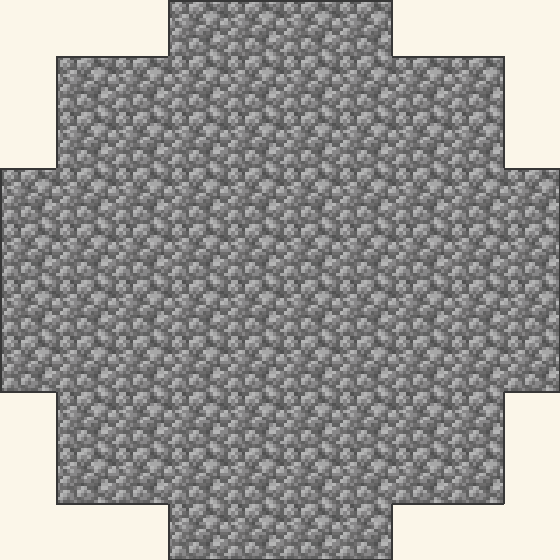
\includegraphics[width=\linewidth]{fig01_2d_d10_euclidean.png}
  \caption{\emph{유클리드}}
\end{subfigure}\hfill
\begin{subfigure}[t]{0.31\linewidth}\centering
  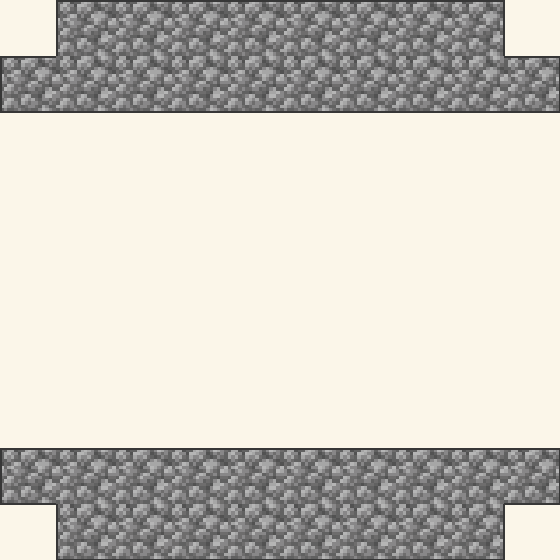
\includegraphics[width=\linewidth]{fig02_2d_d10_bresenham.png}
  \caption{\emph{브레젠험}}
\end{subfigure}\hfill
\begin{subfigure}[t]{0.31\linewidth}\centering
  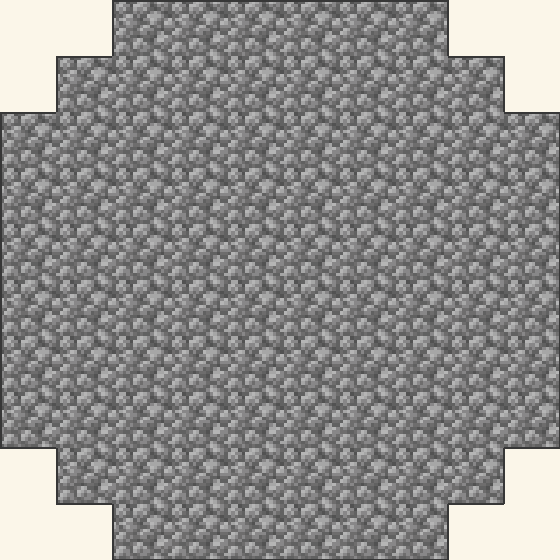
\includegraphics[width=\linewidth]{fig03_2d_d10_threshold.png}
  \caption{\emph{임계값}}
\end{subfigure}
\caption{같은 지름 10의 원이 세 가지 포함 기준에 따라 마인크래프트의 \emph{cobblestone} (둥근돌) 텍스처로 렌더링되었습니다. 모서리 셀, 줄 사이의 전환, 동서남북 점들이 알고리즘마다 어떻게 달라지는지 살펴보세요 --- 세 응답 모두 각자의 기준 아래에서 \emph{수학적으로 옳습니다}. 마인크래프트 건축 계획으로 보면 세 가지가 모두 다른 도면입니다.}
\label{fig:comp-d10}
\end{figure}

\begin{memo}[형평성과 한국 학교 현실]
Block Round의 선택은 한국 교육 환경의 구체적 형평성 문제에도 응답합니다. 한국교육개발원 (KEDI)과 통계청의 자료에 의하면, 한국의 학교 ICT 보급률은 OECD 상위권이지만 학교 간·지역 간 격차가 여전히 존재합니다 (예: 강원도 산간, 전남 도서 지역, 학생수 100명 미만의 농어촌 학교). 반면 청소년의 스마트폰 보유율은 95\% 이상으로 매우 높습니다 (NIA 조사). Block Round는 정확히 이런 환경을 위해 설계되었습니다: 저가 \emph{스마트폰}에서 작동하고, 상시 인터넷이 필요 없으며, 가입도 필요 없습니다. 필요시 부록~\ref{ap:adapt-analog}에 \emph{전적으로 아날로그} 진행 방식 (모눈종이만 사용)도 제공합니다. \emph{마인크래프트 자체 또한 모바일 베드락 에디션이 약 7,900원에 판매되어 매우 접근성이 높습니다}: 학생이 수업에서 Block Round로 시작해 집에서 마인크래프트로 이어갈 수 있습니다.
\end{memo}

\begin{minecraft}[연구: 한국 교육에서의 마인크래프트]
한국에서의 마인크래프트 교육 활용은 점점 확대되고 있습니다. 한국교육학술정보원 (KERIS), 한국교육개발원 (KEDI)의 디지털 교육 보고서, 그리고 SW 교육 의무화 이후 「인공지능 수학」 「정보과」 교과 시범 운영 학교들에서 마인크래프트 에듀케이션 에디션의 활용 사례가 점차 축적되고 있습니다. 「샌드박스 네트워크」 같은 콘텐츠 회사는 마인크래프트 교육 영상의 제작·유통을 담당하며, 일부 시·도 교육청 (특히 서울, 경기)은 「디지털 새싹 교실」 사업의 일환으로 마인크래프트 에듀케이션 활동을 시범 운영하고 있습니다. 마인크래프트 에듀케이션 에디션은 Microsoft 365 Education A1/A3 라이센스로 학교에서 무상 이용 가능합니다 (한국 마이크로소프트 + 교육부 협력). 이 시퀀스는 이러한 전통을 보완합니다: Block Round를 마인크래프트로 가는 \emph{다리}로 활용하여, 수업 중에 게임 설치 (라이선스, 자바, MS 계정 요구 사항)를 면제합니다.
\end{minecraft}

% =============================================================================
\section{학습 목표}\label{sec:objetivos}

\subsection{성취 목표}

학생들은 \acc{이해하고, 비교하고, 활용하고, 건축으로 옮길} 수 있어야 합니다 --- 원, 타원, 타원체의 형식적 정의를 텍스처가 있는 이산 복셀 격자에서의 셀 포함 기준으로 다루며, 이 도형들의 음함수 방정식을 동원하여 \emph{마인크래프트 안에서 건축 가능한} 자작 시각 작품을 설명, 예측, 변형, 제작할 수 있어야 합니다. 한국 시각 문화유산 (단청, 보자기 조각보, 한옥 모듈식 건축, 한국 단색화)과 한국 수학 전통의 대화를 통해 이루어집니다. 다양한 유효 응답의 인식은 \acc{허준이 (June Huh)} 교수가 2022년 한국 출신 최초로 필즈상을 수상한 한국 수학계의 상징적 사건과 연결됩니다 --- 허준이의 사례는 비범한 학교 성적이 아니더라도 세계 최정상 수학자로 성장할 수 있다는 메시지를 한국 사교육 입시 중심 문화에 대한 영감으로 전합니다. 동시에 한국 마인크래프트 커뮤니티는 매일 공간 기하를 실천하면서도 이를 명시적으로 명명하지 않습니다.

\subsection{세부 목표}

\textbf{인지적 (개념적):}
\begin{itemize}[leftmargin=1.3em,itemsep=0.2em,topsep=0.3em]
  \item 음함수 방정식 $\left(\dfrac{x}{r_x}\right)^{\!2} + \left(\dfrac{y}{r_y}\right)^{\!2} = 1$을 원 $x^2 + y^2 = r^2$을 포함하는 일반형으로 인식;
  \item 세 가지 구별되는 포함 기준 (중심점 거리, 브레젠험의 중간점, 모서리 덮음)이 서로 다른 셀 집합을 만들어 낸다는 사실 인식 --- 그림~\ref{fig:comp-d10}에서 이미 본 바와 같이;
  \item 2D 방정식에서 타원체의 3D 방정식으로의 전이를 이해하고 부피 계산 $V = \tfrac{4}{3}\pi r_x r_y r_z$과 연결 (수능 「수학영역」의 미적분/기하 선택 빈출 주제);
  \item 입체를 평면으로 자르는 것을 복셀 좌표에 적용된 \emph{선형 부등식}으로 해석;
  \item \emph{마인크래프트 인벤토리 산술} (스택 64개, 단상자 27 슬롯, 더블 체스트 54 슬롯)을 \emph{올림 나눗셈}과 \emph{몫과 나머지 표현}의 구체적 응용으로 이해;
  \item \cmd{/clone}을 통해 한 팔분원으로부터 완전한 구를 구축하는 \emph{대칭} (반사, 회전)을 인식.
\end{itemize}

\textbf{절차적:}
\begin{itemize}[leftmargin=1.3em,itemsep=0.2em,topsep=0.3em]
  \item Block Round의 인터페이스를 2D와 3D 두 모드에서 조작하고 PNG 이미지와 \texttt{.schem} 스키매틱으로 출력;
  \item 모눈종이 위에 유클리드 기준으로 원의 이산 근사를 손으로 그리고 소프트웨어 결과와 대조;
  \item 셀을 세어 이산 면적/부피를 계산하고 연속 면적/부피와 비교하며 상대 오차로 표현;
  \item 원, 타원, 타원체를 결합한 자작 도형을 수학적 근거로 구성하고 블록 유형별 개수와 더블 체스트 수를 미리 예측;
  \item Block Round가 내보낸 스키매틱을 Litematica 또는 Schematica (마인크래프트 모드)에 임포트하여 게임 안에서 실제로 짓기;
  \item 한 팔분원을 \cmd{/clone}으로 반사하여 완전한 구를 만드는 명령어 시퀀스 작성.
\end{itemize}

\textbf{태도적:}
\begin{itemize}[leftmargin=1.3em,itemsep=0.2em,topsep=0.3em]
  \item 마인크래프트 서버 \emph{빌더} 팀을 본떠 짝 활동·모둠 활동을 통해 협동;
  \item 미적 선택을 수학적으로 옹호 --- 수능 국어와 학생부 종합 전형의 탐구 활동에서 직접 요구되는 역량;
  \item 실제 문제 (「우리 반 마인크래프트 서버에 석영 돔을 짓자」)에 기술적으로 옳은 답이 둘 이상 있음을 인식;
  \item 한국 시각 문화유산, 전통 지혜, 현대 디지털 제작 (서버 \emph{빌더}, 스트리머, 한국 마인크래프트 네트워크)에서 수학적 참조를 발견;
  \item \emph{디지털 윤리} 발전: 동료 작업 존중, 재사용한 \emph{빌드}의 출처 인용, 라이선스 개념 이해.
\end{itemize}

% =============================================================================
\section{2022 개정 교육과정과의 정렬}\label{sec:curriculum}

이 수업 시퀀스는 \acc{2022 개정 초·중등 교육과정} (교육부 고시 제2022-33호, 2024년부터 단계적 시행: 고1은 2025, 고2는 2026, 고3은 2027)의 핵심 역량과 직접 정렬됩니다.

\begin{pyojun}[기하 --- 일반선택]
원, 타원, 쌍곡선, 포물선의 \acc{음함수 방정식}을 다루고 좌표공간에서의 점, 직선, 평면의 위치 관계를 다룹니다. 본 수업은 원과 타원 (2차시), 공간도형과 구의 방정식 (3차시)을 직접 연결합니다.
\end{pyojun}

\begin{pyojun}[미적분 II --- 일반선택]
적분과 \acc{입체도형의 부피}, 회전체의 부피를 다룹니다. 본 수업의 §\ref{aula3}는 타원체 부피 $V = \tfrac{4}{3}\pi r_x r_y r_z$의 \emph{이산 근사}를 통해 적분의 직관적 이해를 보강합니다.
\end{pyojun}

\begin{pyojun}[대수 --- 일반선택]
벡터, 행렬, 일차변환을 다룹니다. 본 수업의 §\ref{aula4} 대칭 \cmd{/clone} 활동은 좌표 반사 ($\mathbb{Z}_2^3$ 군 = 팔분군의 부분군) 변환을 \emph{구체화}합니다.
\end{pyojun}

\begin{pyojun}[인공지능 수학 --- 진로선택]
\acc{데이터의 표현과 처리}, 이미지 데이터, \emph{이산화}, 행렬과 벡터의 응용. 본 수업의 \emph{래스터화} 활동은 이미지를 격자로 표현하는 AI 핵심 개념과 직접 연결됩니다.
\end{pyojun}

\medskip
\emph{교과 핵심 역량}: 문제해결, 추론, 의사소통, 연결, 정보처리; 수학적 모델링 능력. 본 수업은 다섯 역량 모두를 다중적으로 동원합니다.

\subsection{수능과의 연결}\label{sec:suneung}

\acc{대학수학능력시험} (College Scholastic Ability Test, CSAT --- 매년 11월 셋째 주 목요일에 시행)의 수학영역은 학생이 \emph{확률과 통계, 미적분, 기하} 중 하나를 선택해서 응시합니다. 이 중 \emph{미적분}과 \emph{기하}를 선택한 수험생에게는 다음 주제가 본 수업과 직접 관련됩니다:

\begin{itemize}[leftmargin=1.3em,itemsep=0.15em,topsep=0.3em]
  \item \emph{기하}: 원과 타원의 방정식 (포함 기준 = §\ref{aula1}), 공간 좌표 (§\ref{aula3}), 구의 방정식과 평면 (§\ref{aula3} 자르기), 정사영 (§\ref{aula3} 단면).
  \item \emph{미적분}: 적분을 통한 입체도형의 부피 ($V = \int\int\int dV$), 회전체의 부피 (구는 회전체!), 이산 합과 적분의 관계 (§\ref{aula3}).
\end{itemize}

수능 출제 경향상 입체도형의 부피, 좌표공간 점·직선·평면의 관계는 \emph{매년} 1\,~\,2문항씩 출제되는 핵심 영역입니다. 정시와 수시 학생부 종합 전형 모두에서 평가됩니다.

\subsection{디지털 리터러시 정책 정렬}

「2022 개정 초·중등 교육과정 총론」에 따른 \acc{디지털 리터러시 교육}과 「학교 교육과정 편성·운영 지침」의 \emph{AI 교육 강화 정책}을 직접 반영합니다. \emph{디지털 윤리} (자유 소프트웨어와 상용 소프트웨어의 라이선스; Mojang/Microsoft의 마인크래프트 에듀케이션 무상 교육 활용 허용), \emph{개인정보 보호} (\href{https://www.law.go.kr/}{개인정보 보호법 PIPA, 2011년 시행, 2023년 개정}; 정보통신망법; 청소년 보호법), \emph{자작 창작} (5차시에서의 학생 작품 저작권), \emph{디지털 시민의식} (마인크래프트 서버에서의 책임감, 그리핑·온라인 괴롭힘 예방)을 모두 다룹니다.

% =============================================================================
\section{학습 내용}\label{sec:conteudos}

\subsection{개념적 내용}
\begin{itemize}[leftmargin=1.3em,itemsep=0.15em,topsep=0.3em]
  \item $\mathbb{R}^2$와 $\mathbb{R}^3$의 좌표계와 좌표공간; 셀의 \emph{중심} 대 \emph{모서리}.
  \item 원의 표준 방정식: $x^2 + y^2 = r^2$.
  \item 타원의 일반 음함수 방정식: $\left(\dfrac{x}{r_x}\right)^{\!2} + \left(\dfrac{y}{r_y}\right)^{\!2} = 1$.
  \item 포함의 부등식: \emph{내부, 외부, 경계}.
  \item 타원체와 구의 $\mathbb{R}^3$ 방정식.
  \item 타원체의 연속 부피: $V = \tfrac{4}{3}\pi r_x r_y r_z$.
  \item 공간 평면을 선형 부등식으로 (자르기 연산).
  \item 셀의 이웃 (2D는 4-연결, 3D는 6-연결).
  \item \acc{마인크래프트 인벤토리 산술}: 스택 64개; 단상자 (27 슬롯)와 더블 체스트 (54 슬롯); 올림 나눗셈 $N_{\mathrm{packs}} = \lceil N/64 \rceil$.
  \item \acc{팔분 대칭}과 좌표 반사의 $\mathbb{Z}_2^3$ 군 ($O_h$의 위수 8 부분군): \cmd{/clone}을 활용한 최적화된 건축에 응용.
\end{itemize}

\subsection{절차적 내용}
\begin{itemize}[leftmargin=1.3em,itemsep=0.15em,topsep=0.3em]
  \item 명시적 기준에 따른 모눈종이 위의 손 작도.
  \item Block Round 조작 (모드 전환, \emph{슬라이더} 조정, 알고리즘 선택, PNG와 \texttt{.schem} 출력).
  \item 셀 수 세기를 통한 이산·연속 면적과 부피 비교.
  \item 결합 도형의 자작 구성 (\emph{복셀 아트}의 기하학적 정초).
  \item Litematica/Schematica에서 \texttt{.schem} 임포트.
  \item 바닐라 명령어 \cmd{/fill}, \cmd{/clone}, \cmd{/setblock} 실행과 WorldEdit \cmd{//sphere}, \cmd{//hsphere}, \cmd{//ellipsoid}.
  \item 서바이벌 모드 자원 채집 계획.
\end{itemize}

\subsection{태도적 내용}
\begin{itemize}[leftmargin=1.3em,itemsep=0.15em,topsep=0.3em]
  \item 짝과 모둠에서의 협력 작업.
  \item 논거 있는 주장 (수학으로 선택을 정당화).
  \item 디지털 윤리: 소프트웨어 라이선스 존중, 동료 작업 존중, 공유 마인크래프트 서버의 규칙 준수.
  \item 한국 전통 지혜와 현대 \emph{게이머} 문화에 존재하는 수학적 참조를 가치 있게 인식.
\end{itemize}

\subsection{렌더링 모드와 알고리즘의 다양성}

알고리즘 변경 외에도 Block Round는 같은 기하 도형에 대해 시각적으로 다른 결과를 만들어 내는 세 가지 \emph{렌더링 모드} (채움, 얇은, 두꺼운)를 제공합니다 (그림~\ref{fig:render-modes}). 마인크래프트에서 이들은 세 가지 다른 건축 유형에 대응합니다: \emph{채움} 구는 내부 블록을 모두 사용 (속이 채워진 \emph{Stone} 돔); \emph{얇은}은 껍질만 보여줌 (방이나 박물관용 \emph{비어 있는} 돔); \emph{두꺼운}은 얇은 모드가 남기는 대각선 틈새를 메움 (수중의 \emph{유리} 또는 \emph{얼음} 돔이 새지 않도록 만들기 위해 \emph{필수}).

\begin{figure}[!htbp]
\centering
\begin{subfigure}[t]{0.31\linewidth}\centering
  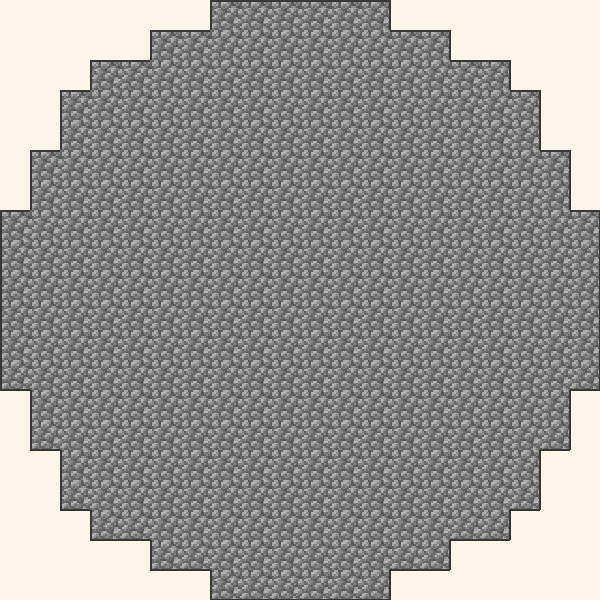
\includegraphics[width=\linewidth]{fig04_2d_d20_euclidean.png}
  \caption{\emph{채움}}
\end{subfigure}\hfill
\begin{subfigure}[t]{0.31\linewidth}\centering
  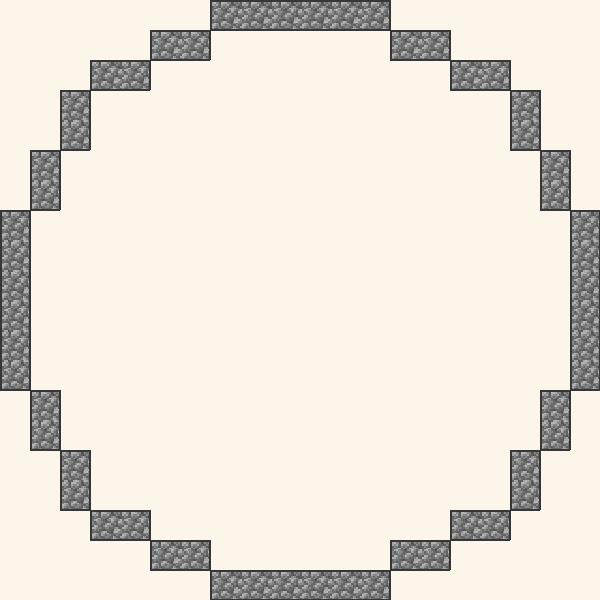
\includegraphics[width=\linewidth]{fig08_2d_d20_thin.png}
  \caption{\emph{얇은} (블록 1개 두께의 윤곽)}
\end{subfigure}\hfill
\begin{subfigure}[t]{0.31\linewidth}\centering
  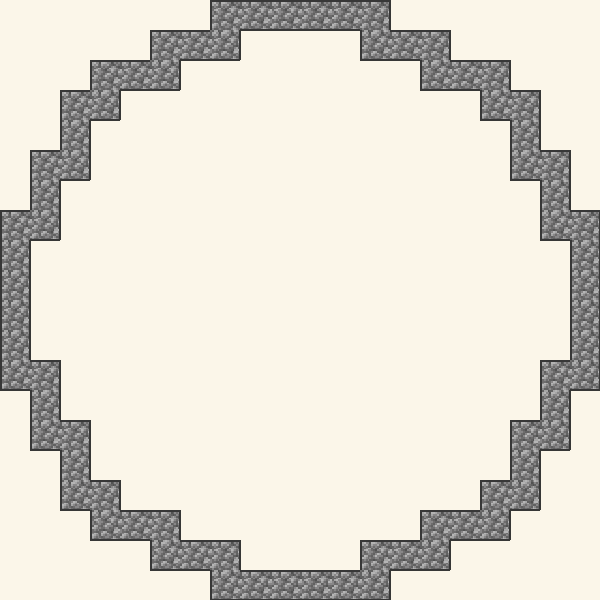
\includegraphics[width=\linewidth]{fig09_2d_d20_thick.png}
  \caption{\emph{두꺼운} (대각 연결을 포함한 윤곽)}
\end{subfigure}
\caption{같은 지름 20의 유클리드 원에 대한 세 가지 렌더링 모드. \emph{얇은} 모드는 위상학적 이산 경계에 대응합니다; \emph{두꺼운} 모드는 대각선 $45^\circ$ 구멍을 피하기 위해 대각선에 블록을 추가합니다 --- 정확히 수중 유리 돔에서 대각선 틈으로 물이 새는 마인크래프트의 실제 문제입니다.}
\label{fig:render-modes}
\end{figure}

\subsection{블록 텍스처: Block Round의 차별점}

\emph{어떤 복셀을 놓을지}의 수학은 텍스처와 무관하지만, Block Round는 각 복셀을 마인크래프트의 정형화된 6면 텍스처로 렌더링합니다. 지름 10의 같은 구도 선택한 블록에 따라 시각적 성격이 완전히 바뀌며 (그림~\ref{fig:textures}), \emph{기반 알고리즘은 전혀 변경되지 않습니다}. 이것이 핵심적인 교육 포인트입니다: \emph{형태}는 수학의 결과이고, \emph{외관}은 그 다음의 미적 결정입니다.

\begin{figure}[!htbp]
\centering
\begin{subfigure}[t]{0.31\linewidth}\centering
  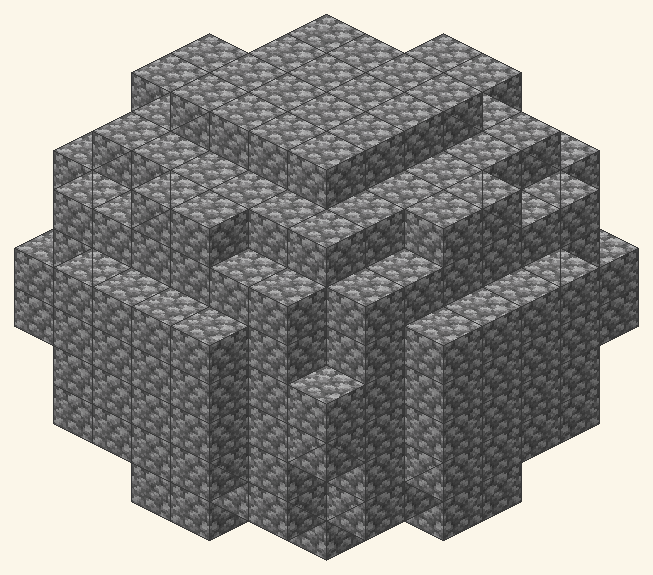
\includegraphics[width=\linewidth]{fig15_3d_sphere_cobblestone.png}
  \caption{\emph{Cobblestone}}
\end{subfigure}\hfill
\begin{subfigure}[t]{0.31\linewidth}\centering
  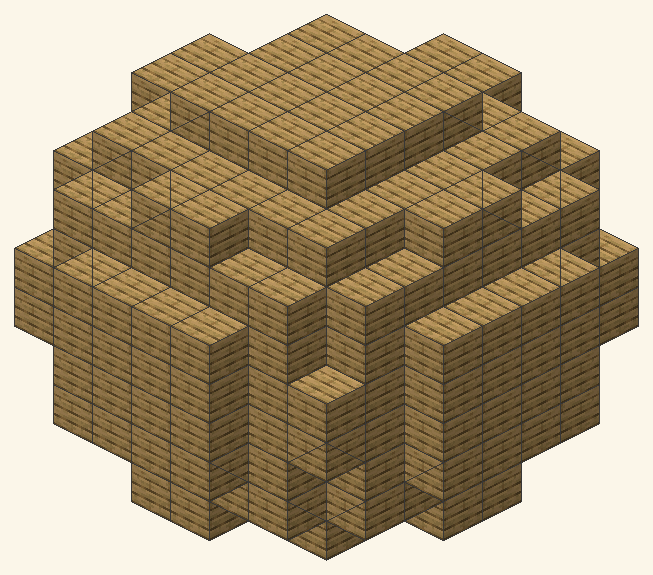
\includegraphics[width=\linewidth]{fig17_3d_sphere_oak.png}
  \caption{\emph{Oak Planks}}
\end{subfigure}\hfill
\begin{subfigure}[t]{0.31\linewidth}\centering
  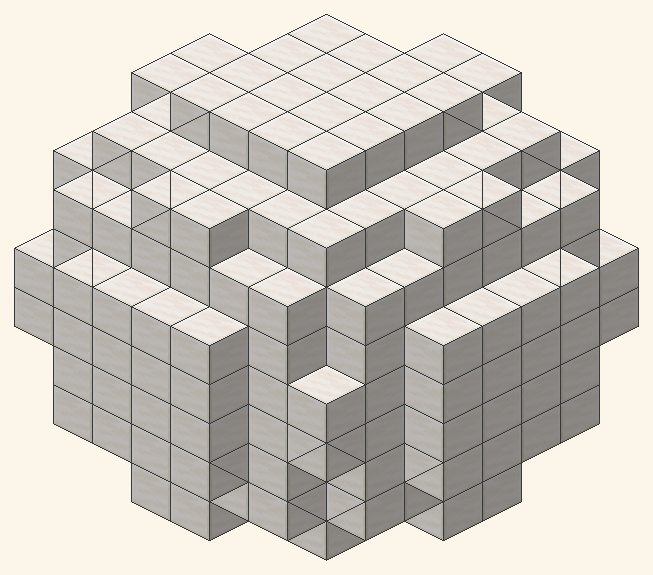
\includegraphics[width=\linewidth]{fig19_3d_sphere_quartz.png}
  \caption{\emph{Quartz Block}}
\end{subfigure}
\caption{지름 10의 \emph{같은} 구에 적용된 세 가지 마인크래프트 텍스처. 복셀화된 실루엣은 세 버전에서 동일합니다 --- 수학이 바뀌지 않았기 때문입니다. 변한 것은 시각적 성격: \emph{Cobblestone}은 중세 성벽을 떠올리게 하고, \emph{Oak Planks}는 한옥 내부나 배 안 같으며, \emph{Quartz Block}은 현대적 사원처럼 보입니다.}
\label{fig:textures}
\end{figure}

% =============================================================================
\section{선수 학습}\label{sec:prerrequisitos}

본 수업은 다음 내용에 대한 사전 학습을 가정합니다:

\begin{itemize}[leftmargin=1.3em,itemsep=0.15em,topsep=0.3em]
  \item 좌표평면과 좌표공간: 점 $(x, y)$와 $(x, y, z)$의 위치.
  \item 원의 표준 방정식 (「공통수학2」 내용).
  \item 다각형의 넓이와 원의 넓이; 정육면체, 각기둥, 원기둥의 부피 (중3·고2 내용).
  \item 함수의 개념: 정의역, 치역, 그래프.
  \item 비례와 백분율.
  \item 정수의 나눗셈 (몫과 나머지) (중학교 내용).
\end{itemize}

\emph{선택적 사전 지식 (필수는 아님):} 마인크래프트 사용 경험. 본 수업은 \emph{전혀} 마인크래프트를 해 본 적이 없는 학생 (드물지만 가능 --- 특히 사교육이나 PC방 접근이 제한된 학생)도 완전히 따라올 수 있도록 의도적으로 설계되었습니다. 모든 조작은 브라우저 안에서 자족적으로 작동하는 Block Round 안에서 이루어집니다.

학급이 위 필수 항목 중 결손을 보일 경우 (코로나19 이후 한국교육과정평가원 (KICE) 및 OECD PISA 결과에서 일부 영역의 격차가 확인됨) --- \emph{1차시}에서 10분의 \emph{진단 평가} 시간을 가집니다 (§\ref{aula1}).

% =============================================================================
\section{자원과 자료}\label{sec:recursos}

\subsection{디지털 자원}
\begin{itemize}[leftmargin=1.3em,itemsep=0.15em,topsep=0.3em]
  \item Block Round (학생 1인당 1개 또는 짝당 1개);
  \item 프로젝터, HDMI 입력 TV 또는 디지털 칠판;
  \item \emph{컴퓨터실} 접근 \emph{또는} 개인 \emph{스마트폰} 사용 (BYOD --- \emph{Bring Your Own Device}) \emph{또는} 시·도 교육청 보급 \emph{태블릿};
  \item (선택, 5차시) \emph{Litematica} 또는 \emph{Schematica} 모드가 설치된 마인크래프트 자바 에디션 또는 마인크래프트 에듀케이션 에디션; 또는 \cmd{/fill}과 \cmd{/clone}으로 바닐라 활용.
\end{itemize}

\subsection{아날로그 자원}
\begin{itemize}[leftmargin=1.3em,itemsep=0.15em,topsep=0.3em]
  \item 모눈종이 (1\,cm), 학생당 2장;
  \item 연필, 지우개, 30\,cm 자;
  \item 색연필 또는 사인펜 (가능하면 풀빛 \texttt{\#5B8E3F}과 흙빛 \texttt{\#825432}, Block Round 색상);
  \item 연습 문제지 (부록~\ref{ap:exerc});
  \item 일반 칠판 또는 화이트보드.
\end{itemize}

\subsection{교과서와 EBS}\label{sec:textbook}

Block Round는 학교 채택 교과서를 \emph{보완}하지 \emph{대체하지} 않습니다. 「2022 개정 교육과정」 검정 교과서 중 본 수업 내용을 다루는 권장 출판사:

\begin{itemize}[leftmargin=1.3em,itemsep=0.1em,topsep=0.2em,nosep]
  \item \emph{고등학교 기하} --- 천재교육, 미래엔, 동아출판, 비상교육, 좋은책신사고, 지학사 (검정 교과서 6종);
  \item \emph{고등학교 미적분 II} --- 동일 출판사들;
  \item \emph{고등학교 인공지능 수학} --- 천재교육, 미래엔, 비상교육 등;
  \item \emph{고등학교 정보} --- 정보과 교과서 (천재교육, 미래엔, 동아출판 등);
  \item EBSi 수능특강 「기하」, 「미적분」 (EBS는 한국 수능 학습의 표준 보조 자료);
  \item EBS \emph{수학의 왕도}, \emph{수능 완성} 시리즈.
\end{itemize}

\emph{원의 방정식}, \emph{이차곡선}, \emph{공간도형}에 대한 단원은 본 수업과 직접 대화합니다. 특히 \emph{타일링}, \emph{덮음}, \emph{격자에서의 세기} 문제 (검정 교과서에 자주 나옴)는 용어만 다를 뿐 Block Round의 핵심 문제와 거의 동일합니다.

\subsection{Block Round 접근}

선호 순서:

\begin{enumerate}[leftmargin=1.5em,itemsep=0.15em,topsep=0.3em]
  \item \textbf{교사가 직접 호스팅}하는 GitHub Pages 또는 학교 포털 (QR 코드로 칠판에 투사). 공개 버전: \url{https://vinisouza128.github.io/block-round/}.
  \item \textbf{프로젝트 파일의 로컬 사본}을 컴퓨터실 폴더에 저장 후 \emph{file://}로 실행.
  \item \textbf{스마트폰 오프라인} (PWA): 인터넷에서 한 번 열면 브라우저가 앱을 설치.
\end{enumerate}

% =============================================================================
\section{한국 교육 현장의 다양성에 따른 적용}\label{sec:adapt}

한국의 고등학교는 다양합니다 --- 학교 유형, 지역, 학생 구성, 시설 수준에서. 이 시퀀스는 그러한 다양성을 위해 설계되었으며, 각 맥락에 따른 변형을 제시합니다.

\subsection{수도권/광역시 일반고등학교}
서울, 부산, 대구, 인천, 광주, 대전, 울산, 세종 등의 일반고. 일반적으로 컴퓨터실 (공동 사용), 디지털 칠판, Wi-Fi가 충분히 갖춰져 있습니다. 많은 학교가 \emph{마인크래프트 에듀케이션 에디션}을 학생에게 라이선스하므로, 5차시는 그 안에서 통째로 진행할 수 있습니다. \emph{시퀀스 전체를 컴퓨터실에서 가장 쉽게 구현할 수 있는 환경.}

\subsection{중소도시 / 군 단위 일반고}
한국 대다수 시·군의 현실입니다. 컴퓨터실이 부분 가동 중일 수 있습니다. 학생의 개인 \emph{스마트폰}을 사용하는 \emph{BYOD 모델}을 권장하며, 짝별로 1대씩 (총 학급당 15~20대) 운용합니다. Block Round는 2018년 이후 출시된 \emph{Android}와 iPhone에서 편안하게 작동합니다. \emph{마인크래프트} 사용이 불가능하면 5차시를 가상 명령어 (종이 + 효과 설명)로 진행해도 개념 내용을 잃지 않습니다. 한국에서 \acc{가장 빈도가 높은} 환경입니다.

\subsection{특수목적고 / 마이스터고 / 자율형 사립고}
외국어고 (외고), 과학고 (전국 20여 개교), 한국과학영재학교 (KSA), 영재학교 (전국 8개교), 예술고, 체육고, 마이스터고 (산업수요맞춤형고 50여 개교 --- IT, 반도체, 자동차, 게임 분야), 특성화고, 자율형 사립고 (자사고), 자율형 공립고. 시설이 매우 충실하고 학생의 ICT 활용 능력이 높습니다. 시퀀스는 자연스럽게 통합과정 (정보과, 디지털컴퓨터 통합, 게임 디자인)과 결합됩니다. 2차시 (브레젠험 알고리즘)는 컴퓨터실에서 Python 구현으로 심화하기를 권장하며, 5차시는 학교 서버에 실제 마인크래프트 자바 서버를 설치하여 협동 건축을 진행할 수 있습니다 --- KSA, 영재학교, 마이스터고 (게임 콘텐츠과)의 자율탐구 활동·동아리 활동과 직접 연계됩니다.

\subsection{농산어촌 · 도서벽지 학교}
강원도 산간, 전남 도서 (완도·신안·진도), 제주 일부, 학생수 100명 미만의 작은 학교. 디지털 시설이 상대적으로 부족할 수 있지만 학생의 \emph{공간적 직관과 모듈식 사고력}이 강한 경우가 많습니다 (예: 농작물 배치, 한옥 칸 단위 구조, 어선의 그물 격자, 산간의 다랑이 논 = 직접 voxel!). 아날로그 변형 (부록~\ref{ap:adapt-analog})과 교사 1대의 시연 기기를 권장합니다. 3차시는 학생이 잘 아는 농가의 둥근 곡식 창고, 모듈식 비닐하우스, 한옥 구조 등을 활용해 \emph{몸으로 산 기하}와 \emph{기호의 기하}를 잇습니다.

\subsection{다문화 학생 비율이 높은 학교}
경기 안산, 시흥, 화성, 서울 영등포·구로 등 다문화 학생 비율이 높은 지역의 일반고. 「다문화학생 교육지원」 정책 대상 학교. 다문화 가정 학생, 외국인 노동자 자녀, 북한이탈주민 자녀, 결혼이주여성 자녀 등이 함께 학습합니다. Block Round는 시각 자료가 많고 한국어 텍스트가 적어 접근성이 좋습니다. 부록 활동에 다양한 문화 (몽골 게르의 둥근 천장, 베트남 모자의 원뿔, 우즈베키스탄 차도르 패턴 등)를 반영해 학급의 문화 다양성을 자원으로 삼을 수 있습니다.

\subsection{학생수 급감 지역 학교 (지방소멸 위험지역)}
지방소멸 위험지역의 농어촌 학교, 학교 통폐합 대응 지역. 학급당 학생 수가 10명 이하인 \emph{초소형 학교}. 이 경우 \emph{개별화} (학생당 1대) 학습이 가능하므로 Block Round의 효과가 극대화됩니다. 통폐합으로 인한 학교 정체성 위기를 \emph{건축적 자기 표현} (5차시 「우리 학교를 마인크래프트로 짓기」)으로 전환하면 의미 있는 교과 활동이 됩니다.

\subsection{방송통신고 / 평생교육 시설 / 검정고시 학원}
방송통신고등학교 (방통고), 평생교육 시설, 학력인정 평생교육시설, 검정고시 학원 (Korean GED 등가). 성인 학습자 또는 학교 부적응 청소년의 대안 경로. Block Round의 인터페이스가 친절하고 마인크래프트의 청소년 친화적 특성이 성인 학습자에게도 좋습니다 (대부분 자녀가 마인크래프트를 하므로 친숙). 각 활동을 20\% 줄여 진행 (수업 시간이 학교보다 짧음)하고, 긴 서술형 대신 토의 중심으로 변형하기를 권장합니다. 5차시는 \emph{선택 활동}으로 두고 1~4차시를 핵심으로 잡습니다.

\subsection{2시간 블록 시간표 변형 (100분 단위)}
이중 모듈 시간표 학교 (마이스터고, 일부 자사고)의 경우: 1+2차시를 한 모듈, 3+4차시를 다음 모듈, 5차시는 단독 (50분 혹은 100분 또는 200분 블록 — 실제 마인크래프트 건축 시간 확보). 총: 100분 모듈 3개 + 50분 1개, 또는 100분 모듈 2개 + 200분 블록 1개 (마지막 실습용).

\subsection{시·도 교육청 교육과정과의 연계}

각 시·도 교육청은 2022 개정 교육과정을 자체 특색사업과 결합하여 운영합니다. 주요 사례:

\begin{center}
\small
\begin{tabularx}{\textwidth}{@{}p{0.22\textwidth}p{0.26\textwidth}X@{}}
\toprule
\textbf{교육청} & \textbf{주요 특색사업} & \textbf{본 수업과의 연계점} \\
\midrule
서울특별시교육청 & 디지털 새싹 교실, AI 교육 강화 & 인공지능 수학 + 기하 통합; \emph{서울 디지털 트윈}과 voxel 연결 \\
\addlinespace[3pt]
경기도교육청 & IB (국제 바칼로레아) 도입, 학생 수 전국 최대 & MYP/DP 수학 탐구활동 (Internal Assessment)으로 5차시 활용 \\
\addlinespace[3pt]
부산광역시교육청 & 해양 · 항만 · 조선 산업 연계 & 부산 누리마루, 영화의 전당 같은 곡선 건축 사례 \\
\addlinespace[3pt]
강원특별자치도교육청 & 농산어촌 학교 통폐합 대응 & 작은 학교 개별화 활용; 너와집·산간 한옥 사례 \\
\addlinespace[3pt]
전라남도교육청 & 도서 · 다문화 교육 & 도서 지역 PWA 오프라인 활용; 다문화 학생 통합 \\
\addlinespace[3pt]
제주특별자치도교육청 & 도서 + 영어교육도시 & 통가옥·돌담과 voxel 연결; 영어 자료 활용 \\
\addlinespace[3pt]
충청남도교육청 & 마이스터고 산업 연계 (반도체, 자동차) & 마이스터고 학생을 위한 Python·정보과 심화 \\
\bottomrule
\end{tabularx}
\end{center}

\subsection{온라인 · 원격 학습 환경}
Block Round의 \emph{웹} 기반 특성은 원격 수업 (\emph{Zoom for Education}, \emph{e-학습터}, \emph{EBS 온라인 클래스}, \emph{클래스팅}, \emph{카카오 클래스룸})에 자연스럽게 호환됩니다. 교사가 화면 공유하면 학생은 자기 기기에서 따라 옵니다. 모눈종이 활동은 사진 촬영하여 카카오톡 단톡, 구글 클래스룸 또는 학교 LMS에 비동기 과제로 제출할 수 있습니다. 5차시는 공유 마인크래프트 서버 (\emph{Realms} 또는 자체 서버)에서 학급 전체가 가상 세계에서 만나 협동 건축을 진행할 수 있습니다. \emph{디지털 교과서} 보급 학교에서는 디지털 교과서 안의 시뮬레이션 도구와도 결합 가능합니다.

% =============================================================================
\section{수업 시퀀스}\label{sec:sequencia}

본 시퀀스는 \acc{동기 유발 --- 문제 제기 --- 개념 정리 --- 종합}의 구조를 따르며, 한국 수학교육학회와 대한수학교육학회 연구자들이 권장하는 \emph{문제 해결 학습 모형}, Bruner의 \emph{발견 학습 모형}, 그리고 자기주도학습 (셀프-디렉티드 러닝)의 한국 교육 전통에 기반합니다. 50분 차시마다 청소년의 인지 리듬을 고려하여 짧은 강의 ($\leq 15$\,분)와 실습 활동을 교차시킵니다.

% =============================================================================
\subsection{1차시 --- \enquote{게임은 어떻게 구로 구를 그릴까?}}\label{aula1}

\subsubsection*{차시 목표}
이산 래스터화의 \emph{핵심 문제}를 진정한 수학 문제로 설정하고, 원의 방정식을 동원하며 Block Round를 소개합니다. 차시의 핵심 문제 --- \emph{어떤 블록을 칠할지 어떻게 결정할까?} --- 가 마인크래프트로 구를 만드는 모든 플레이어가 부딪히는 그 문제임을 인식합니다.

\begin{hwaldong}[1.1 --- 동기 유발 \quad\tempo{10분}]
\textbf{전략:} \emph{think--pair--share} (개별 사고, 짝 대화, 학급 공유). \\[0.4em]
\textbf{단계:}
\begin{enumerate}[leftmargin=1.5em,itemsep=0.2em,topsep=0.3em,nosep]
  \item 마인크래프트의 고전적 건축 세 가지를 투사 (또는 그림으로 제시): \emph{Stone} 토대 위 \emph{Glass} 돔; 한국 마인크래프트 서버 (또는 양띵·우왁굳·풍월량 같은 한국 스트리머의 영상)에 등장하는 \emph{거대 구}; 한국 청소년 픽셀 아트 (BTS 멤버, 「오징어 게임」 캐릭터, 「뽀로로」, K-pop 아이돌 등).
  \item 학급에 묻기: \emph{\enquote{잘 보세요. 이 게임은 어떻게 구를 그릴 블록들을 정할까요? 마인크래프트 안에 \enquote{마법 컴퍼스}가 들어 있을까요?}}
  \item 각 학생이 1분 동안 개별적으로 답을 적고, 옆 짝과 2분 동안 의견을 나눕니다.
  \item 집단 수렴: 핵심 응답을 칠판 한쪽에 정리. 근본적 관찰로 유도: \emph{\enquote{게임은 완전한 정육면체만 놓을 수 있어요 --- 어떻게 어떤 큐브를 놓을지 결정할까요?}}
\end{enumerate}
\end{hwaldong}

\begin{hwaldong}[1.2 --- 문제 제기 \quad\tempo{15분}]
\textbf{전략:} 손 작도와 형식적 정의의 대결. \\[0.4em]
\textbf{준비물:} 모눈종이, 연필. \\[0.4em]
\textbf{단계:}
\begin{enumerate}[leftmargin=1.5em,itemsep=0.2em,topsep=0.3em,nosep]
  \item 각 학생에게 모눈종이 반 장 배부, $11 \times 11$ 영역의 중심 점을 표시.
  \item 지시: \emph{\enquote{여러분이 만들 수 있는 가장 좋은 지름 10 (반지름 5)의 원을 그려 보세요. \emph{각 칸이 마인크래프트의 cobblestone 블록 1개라고 생각하세요.} 시간은 4분입니다.}}
  \item 시간 후, 학생 3~4명이 자신의 그림을 칠판의 격자 (분필이나 마커로 그린)에 옮겨 그립니다.
  \item 교사 유도 관찰: \emph{\enquote{보세요. 모두 같은 그림인가요? 왜 다른가요? 누가 맞나요? 만약 여러분이 마인크래프트 공유 서버에서 이 구를 함께 짓고 있다면, 이런 차이가 어떤 문제를 일으킬까요?}}
  \item 정리: \emph{유일한} 답은 없습니다 (§\ref{sec:justificativa}에서 본 그림~\ref{fig:comp-d10}이 이를 뒷받침합니다). 각 학생은 셀의 포함 여부를 결정하는 \acc{기준}을 암묵적으로 다르게 채택했습니다.
\end{enumerate}

\textbf{한국 마인크래프트 커뮤니티 노트:} 이 다양한 응답 자체가 \emph{문화적으로 흥미로운 현상}임을 언급합니다. 한국 마인크래프트 커뮤니티 (양띵, 우왁굳, 풍월량, 침착맨, 「샌드박스 네트워크」 등의 채널)는 한국어로 된 둥근 건축 튜토리얼을 자주 만들며, 각자 약간씩 다른 \emph{경험적 비법}을 전수합니다. 이 비법들은 사실상 서로 다른 「민족수학」 — 알고리즘 — 입니다.
\end{hwaldong}

\begin{hwaldong}[1.3 --- 개념 정리 \quad\tempo{15분}]
\textbf{전략:} 칠판을 활용한 대화형 강의. \\[0.4em]
\textbf{내용:}

원점을 중심으로 반지름 $r$인 원의 음함수 방정식:

\begin{susik}
\centering
$\displaystyle x^2 + y^2 \;=\; r^2$
\end{susik}

\emph{내부}의 점은 $x^2 + y^2 < r^2$을 만족; \emph{외부}는 $x^2 + y^2 > r^2$. 이 방정식은 반축 $r_x, r_y$의 타원으로 일반화됩니다:

\begin{susik}
\centering
$\displaystyle \left(\dfrac{x}{r_x}\right)^{\!2} + \left(\dfrac{y}{r_y}\right)^{\!2} \;=\; 1$
\end{susik}

블록 (복셀) 격자에서는 어떤 \acc{셀}을 내부에 포함시킬지 결정해야 합니다. 결정이 다르면 도면이 달라집니다. Block Round는 \emph{세 가지} 기준을 구현합니다:

\begin{itemize}[leftmargin=1.3em,itemsep=0.15em,topsep=0.3em]
  \item \acc{유클리드}: 셀의 중심 $(i + \tfrac{1}{2},\, j + \tfrac{1}{2})$이 내부에 있는가?
  \item \acc{브레젠험}: 1965년 IBM의 Jack Bresenham이 개발한 역사적 알고리즘, 정수 연산만으로 작동.
  \item \acc{임계값}: 셀의 한 \emph{모서리}가 내부에 있는가?
\end{itemize}

\textbf{시연:} 교사가 Block Round를 열어 지름을 10으로 맞추고, 학급이 차이를 관찰하는 동안 세 알고리즘을 번갈아 적용합니다. 강조: 세 도면은 서로 다른 기준 아래에서 모두 \emph{수학적으로 옳습니다}. 앱이 블록 텍스처를 바꿀 수 있음을 보여줍니다 --- 구가 cobblestone, oak\_planks, diamond, glowstone으로 차례로 변하되 형태는 \emph{변하지 않음}. \emph{이것이 Block Round의 핵심 포인트: 형태는 수학, 텍스처는 미적 선택.}
\end{hwaldong}

\begin{hwaldong}[1.4 --- 종합 \quad\tempo{10분}]
\textbf{전략:} 즉각적 개별 응용. \\[0.4em]
\textbf{지시:} \emph{\enquote{종이로 돌아가세요. 유클리드 기준을 \acc{엄격하게} 적용해 지름 10의 원을 다시 그리세요: 셀의 중심점 $(i + 0{,}5,\, j + 0{,}5)$이 중심으로부터 거리 5 이하인 경우에만 그 셀을 칠합니다.}}

활동 끝에 종이의 그림을 Block Round의 지름 10 유클리드 알고리즘 결과와 비교 --- 시각 참조는 그림~\ref{fig:comp-d10}~(a). \emph{일치해야 합니다.}
\end{hwaldong}

\begin{minecraft}[게임과의 연결]
WorldEdit 모드가 설치된 \emph{마인크래프트 자바 에디션}에서 \cmd{//sphere stone 5} 명령은 Block Round의 \emph{브레젠험} 알고리즘이 지름 10에서 만드는 도면과 동일한 도면을 만듭니다. 서버에서 게임하는 학생들은 집에서 이를 확인할 수 있습니다 --- 건축이 동일합니다. \emph{즉, 우리가 수업에서 공부하는 내용은 마인크래프트를 위한 시뮬레이션 학습이 아닙니다. 게임 자체가 사용하는 그 수학입니다.}
\end{minecraft}

\subsubsection*{과제 (선택)}
연습 1.4를 지름 8과 14로 반복. 다음 시간에 세 그림을 가져옵니다. 집에서 마인크래프트를 하는 학생은: 그림을 게임 안에서 직접 재현 (\cmd{/setblock}으로 블록 단위, 또는 WorldEdit이 있으면 \cmd{//sphere}로) 후 사진 촬영.

% =============================================================================
\subsection{2차시 --- \enquote{세 알고리즘, 세 도면, 세 건축 계획}}\label{aula2}

\subsubsection*{차시 목표}
세 알고리즘을 수학적으로 구별된 정의로 깊이 이해하고, 결과를 정량적으로 비교합니다 --- 서바이벌 빌더 관점에서 \emph{채집해야 할 블록 개수}의 실질적 영향까지 포함합니다.

\begin{hwaldong}[2.1 --- 회고 \quad\tempo{5분}]
지난 시간 과제 그림을 빠르게 수거, 학급 내 변이를 관찰, 차시 목표 안내: \emph{\enquote{오늘은 세 알고리즘 하나하나를 돋보기로 들여다보고, 왜 브레젠험이 컴퓨팅 분야의 보석이라 불리는지 --- 그리고 한국 마인크래프트 커뮤니티가 브레젠험이라는 이름을 한 번도 들어본 적 없으면서도 매일 그를 사용하는 이유를 발견합시다.}}
\end{hwaldong}

\begin{hwaldong}[2.2 --- 유클리드 알고리즘 \quad\tempo{10분}]
형식화. 셀 $(i, j)$에 대해 정규화된 좌표 계산:

\begin{susik}
\centering
$\displaystyle d_x = \dfrac{i + \tfrac{1}{2} - c_x}{r_x},\qquad d_y = \dfrac{j + \tfrac{1}{2} - c_y}{r_y}$
\end{susik}

셀은 $d_x^{\,2} + d_y^{\,2} \leq 1$일 때만 칠해집니다.

\textbf{칠판:} $c_x = c_y = 5$, $r_x = r_y = 5$, 셀 $(2, 1)$의 경우를 명시적으로 풀이. $d_x = (2{,}5 - 5)/5 = -0{,}5$, $d_y = (1{,}5 - 5)/5 = -0{,}7$, 따라서 $d_x^2 + d_y^2 = 0{,}25 + 0{,}49 = 0{,}74 \leq 1$. 셀 \emph{내부}. \\

학생에게 셀 $(0, 0)$을 시험 (결과는?) 후 토론.
\end{hwaldong}

\begin{hwaldong}[2.3 --- 브레젠험 알고리즘 \quad\tempo{15분}]\label{at:23}
\textbf{역사적 맥락:} Jack Bresenham은 1965년 IBM 재직 시 알고리즘을 발표했습니다. 그 이전에는 직선 작도가 부동소수점 연산을 요구했고, 이는 당시 컴퓨터에서 비용이 매우 컸습니다. Bresenham은 \emph{정수만으로} 작도 가능함을 보였습니다: 덧셈과 비교만으로.

원에 대한 변형은 \emph{결정 매개변수} $d$를 사용합니다. $(x{=}0,\, y{=}R)$에서 $d_0 = 1 - R$로 시작. $0$--$45^\circ$ 팔분원에서 각 단계:

\begin{susik}
\centering
$\begin{cases}
\text{만약 } d < 0: & \text{다음: } (x{+}1,\, y),\; d \mathrel{+}= 2x+3 \\
\text{만약 } d \geq 0: & \text{다음: } (x{+}1,\, y{-}1),\; d \mathrel{+}= 2(x-y)+5
\end{cases}$
\end{susik}

\textbf{칠판 시연:} $R = 5$에 대해 알고리즘을 한 단계씩 추적하며 각 반복의 $x, y, d$를 기록. 여덟 팔분원은 대칭으로 얻음. \\

\textbf{마인크래프트와의 연결:} WorldEdit 모드의 \cmd{//sphere} 명령 (Sponge, Bukkit, Paper, Fabric)은 브레젠험 3D의 변형을 구현 --- 1965년의 같은 수학이 전 세계 수백만 마인크래프트 서버에서 작동합니다. \emph{여러분이 지금 배우는 것은 누군가 \texttt{//sphere stone 8}을 입력할 때마다 게임이 내부에서 사용하는 수학입니다.}

\textbf{한국정보올림피아드 (KOI)와의 연결:} 브레젠험 알고리즘은 \href{https://www.digitalculture.or.kr/koi/}{한국정보올림피아드 (KOI)}와 알고리즘 챔피언십 출제의 고전 주제입니다. 한국정보화진흥원 (NIA)이 주관하며 국제정보올림피아드 (IOI) 한국 대표를 선발합니다. 관심 학생은 KOI 포털 무료 자료로 심화 학습 가능.

\textbf{수업 방법 메모:} 학급이 매개변수 $d$의 대수에 어려움을 보이면 알고리즘을 단순 \emph{규칙}으로 제시하고 (결정 함수의 유도는 생략) 정당화는 기술 문서 \texttt{Block\_Round\_Math\_ko-KR.pdf} §5를 참조하면 충분합니다.
\end{hwaldong}

\begin{hwaldong}[2.4 --- 임계값 알고리즘 \quad\tempo{10분}]
각 셀 $(i, j)$에 대해 형태 중심에 \emph{가장 가까운 모서리}를 식별:

\begin{susik}
\centering
$\displaystyle n_x = \mathrm{clamp}(c_x,\, i,\, i{+}1),\qquad n_y = \mathrm{clamp}(c_y,\, j,\, j{+}1)$
\end{susik}

셀은 $\left(\dfrac{n_x - c_x}{r_x}\right)^{\!2} + \left(\dfrac{n_y - c_y}{r_y}\right)^{\!2} \leq 0{,}94$일 때 포함됩니다.

\textbf{왜 $1$이 아니라 $0{,}94$인가?} 경험적으로 $1$을 사용하면 동서남북 방향에 1블록 \emph{가시}가 생깁니다. 약간 작은 임계값은 이 잘못된 모양을 제거합니다. \emph{이론적 수학만으로 부족할 때 기술적 결정이 시각 검토를 통해 보완되는 사례입니다} --- 이론과 실천의 대화를 보여 줍니다. 한국 수학교육 전통에서 강조되는 \emph{탐구학습}과 \emph{귀납적 발견}의 관점에 부합합니다.

\textbf{마인크래프트에서 임계값을 언제 쓰는가:} \emph{멀리서 보는} 돔과 봉우리 (산 위의 사원, 섬의 묘소)에 임계값 알고리즘은 약간 \emph{더 가득찬} 실루엣을 만들어 안개와 환경광 차폐를 뚫고 더 잘 읽힙니다. 비용: 껍질당 약 5--10\% 블록 추가. 멀리서 보는 미학이 자재 절감보다 더 중요한 프로젝트에 권장.
\end{hwaldong}

\begin{hwaldong}[2.5 --- 정량 비교 \quad\tempo{10분}]\label{at:25}
\textbf{짝 활동.} Block Round (또는 중앙 프로젝터)에서:
\begin{enumerate}[leftmargin=1.5em,itemsep=0.15em,topsep=0.3em,nosep]
  \item 지름 20과 \emph{채움} 모드 설정 (그림~\ref{fig:comp-d20}은 각 알고리즘의 예상 결과).
  \item 캔버스 모서리의 \emph{Info chip} 작동. 세 알고리즘 각각의 면적 기록.
  \item 연속 면적 계산: $\pi r^2 = \pi \cdot 10^2 \approx 314{,}16$.
  \item 각 알고리즘에 대해 상대 오차 계산: $\dfrac{|\text{이산 면적} - \text{연속 면적}|}{\text{연속 면적}} \times 100\%$.
  \item 세 알고리즘을 연속값으로부터 가장 가까운 것부터 가장 먼 것 순으로 정렬.
  \item \emph{마인크래프트와의 연결:} \enquote{\emph{여러분이 이 세 구를 서바이벌에서 짓는다면, 어느 것이 cobblestone 창고 왕복을 가장 적게 요구할까요? 어느 것이 가장 많을까요?}} 최소 면적 알고리즘 (유클리드)과 최대 면적 알고리즘 (임계값) 사이의 \emph{스택} (64 블록) 차이는 한 스택 전체에 이를 수 있습니다.
\end{enumerate}

\textbf{예상 결과:} 유클리드는 매우 근접 (오차 2\% 이하); 임계값은 몇 \%로 과대; 브레젠험은 그 사이. 집단 확인.
\end{hwaldong}

\begin{figure}[!htbp]
\centering
\begin{subfigure}[t]{0.31\linewidth}\centering
  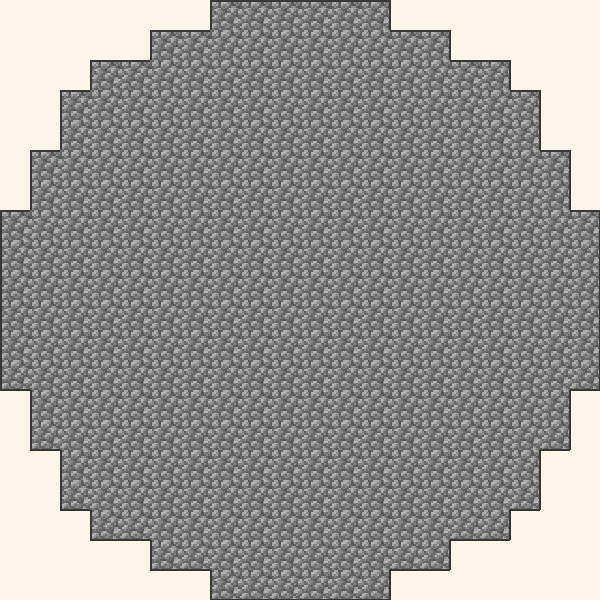
\includegraphics[width=\linewidth]{fig04_2d_d20_euclidean.png}
  \caption{\emph{유클리드}}
\end{subfigure}\hfill
\begin{subfigure}[t]{0.31\linewidth}\centering
  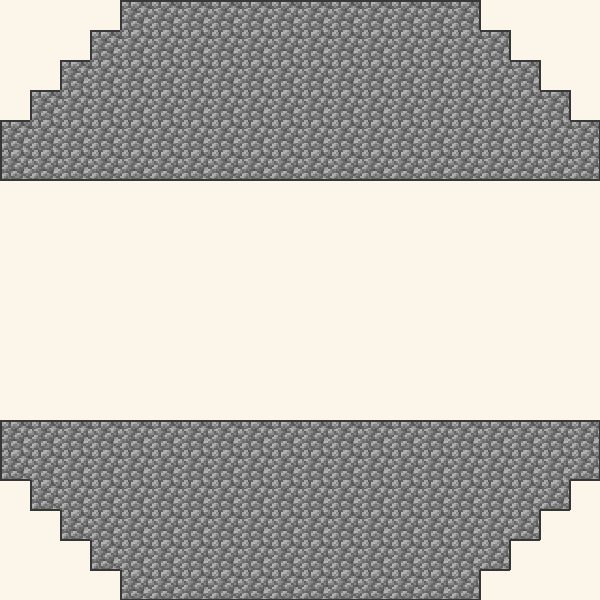
\includegraphics[width=\linewidth]{fig05_2d_d20_bresenham.png}
  \caption{\emph{브레젠험}}
\end{subfigure}\hfill
\begin{subfigure}[t]{0.31\linewidth}\centering
  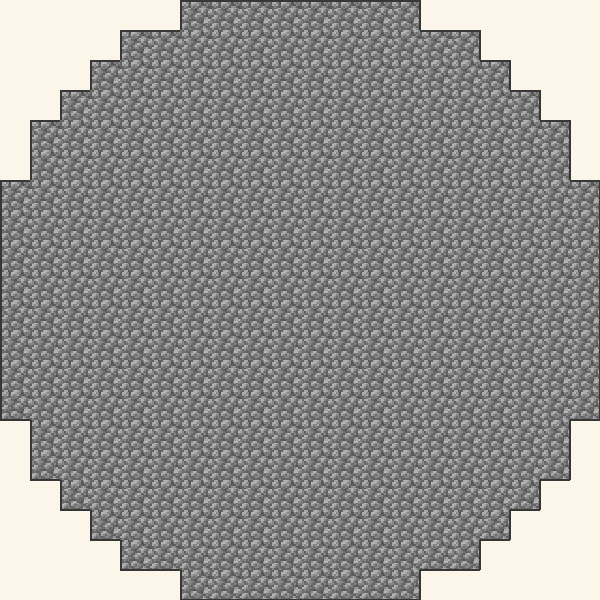
\includegraphics[width=\linewidth]{fig06_2d_d20_threshold.png}
  \caption{\emph{임계값}}
\end{subfigure}
\caption{cobblestone 텍스처로 렌더링된 세 알고리즘에서의 같은 지름 20 원. 지름이 커지면 차이가 보다 미묘해져 세 버전이 육안으로 비슷해 보입니다. 작은 지름 (그림~\ref{fig:comp-d10})에서 차이가 훨씬 명백하다는 점을 짚어 주기 좋은 순간입니다.}
\label{fig:comp-d20}
\end{figure}

\begin{minecraft}[블록 비교: Block Round 대 WorldEdit]
집에서 시도 (마인크래프트 + WorldEdit 있다면): 서버에서 \cmd{//sphere stone 10}을 실행하고 블록을 세어 보세요. 그리고 Block Round의 브레젠험 알고리즘 $D = 20$의 \emph{Info chip}이 표시하는 수와 비교. 두 수치는 일치해야 합니다 (\emph{또는} 작은 구현 차이로 0--4 블록 정도 차이). 일관된 차이를 발견한다면 진짜 수학적 호기심을 발견한 것입니다.
\end{minecraft}

% =============================================================================
\subsection{3차시 --- \enquote{타원에서 타원체로: 3차원}}\label{aula3}

\subsubsection*{차시 목표}
타원 방정식을 타원체로 일반화, 복셀·이산 부피·평면 자르기를 도입. 한국 시각 전통 및 한국 마인크래프트 커뮤니티의 유명 건축물과 다리를 놓습니다.

\begin{hwaldong}[3.1 --- 2D 방정식에서 3D로 \quad\tempo{15분}]\label{at:31}
좌표평면에 세 번째 좌표 $z$를 더합니다. 타원의 음함수 방정식은 자연스럽게 일반화됩니다:

\begin{susik}
\centering
$\displaystyle \left(\dfrac{x}{r_x}\right)^{\!2} + \left(\dfrac{y}{r_y}\right)^{\!2} + \left(\dfrac{z}{r_z}\right)^{\!2} \;=\; 1$
\end{susik}

$r_x = r_y = r_z = r$일 때, \acc{구} $x^2 + y^2 + z^2 = r^2$를 회복합니다 (그림~\ref{fig:3d-shapes}).

\textbf{복셀:} 3D 격자의 셀은 \emph{복셀} (\emph{volume element})이라 부릅니다. 마인크래프트에서 각 복셀은 $1\times1\times1$ \emph{블록}에 해당합니다. 포함 기준은 2D의 것에 $z$ 좌표를 더한 것과 정확히 동일:

\begin{susik}
\centering
$\displaystyle a_x^2 + a_y^2 + a_z^2 \leq 1,\quad \text{여기서 } a_\xi = \dfrac{\xi + \tfrac{1}{2} - c_\xi}{r_\xi}$
\end{susik}

\textbf{시연:} Block Round를 3D 모드로 열고 구와 타원체를 번갈아 보여 줌. \emph{마우스}로 회전, 복셀 구조 관찰.
\end{hwaldong}

\begin{figure}[!htbp]
\centering
\begin{subfigure}[t]{0.45\linewidth}\centering
  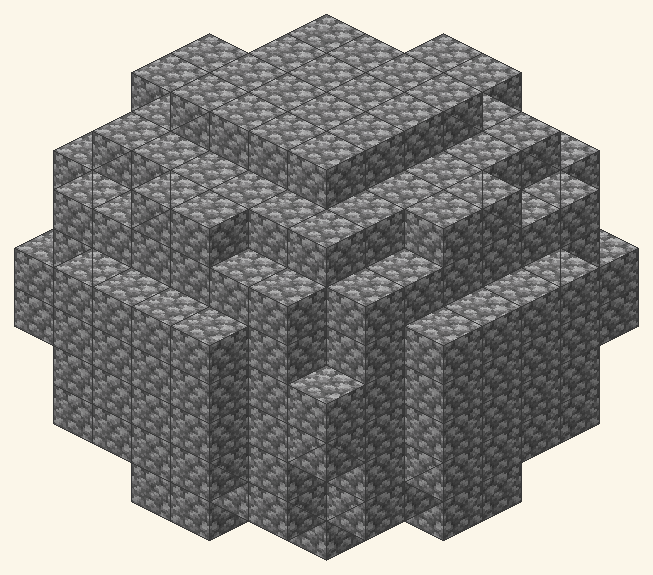
\includegraphics[width=\linewidth]{fig10_3d_sphere_d12.png}
  \caption{지름 10의 구 ($r_x = r_y = r_z = 5$).}
\end{subfigure}\hfill
\begin{subfigure}[t]{0.45\linewidth}\centering
  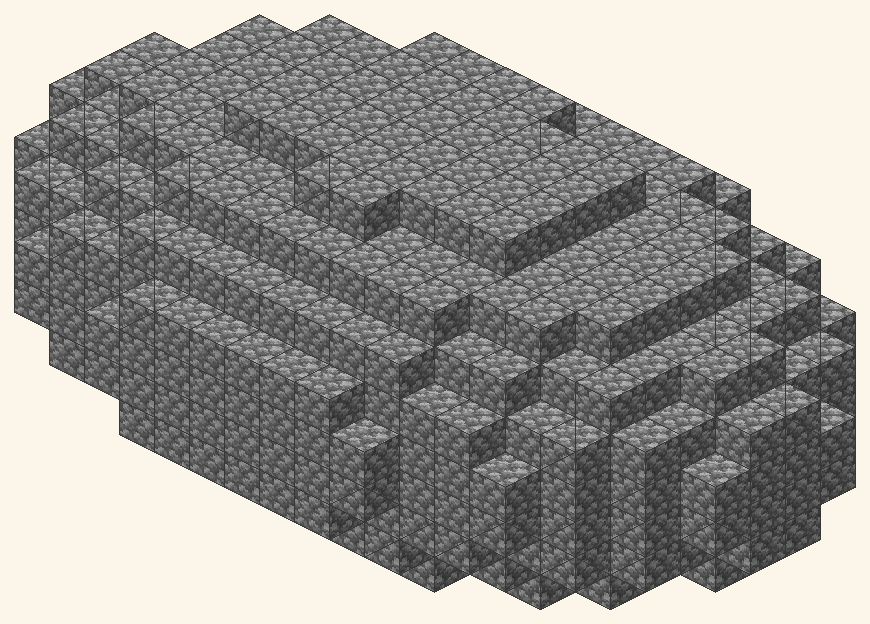
\includegraphics[width=\linewidth]{fig11_3d_ellipsoid.png}
  \caption{$W = 20, H = 10, D = 12$의 타원체.}
\end{subfigure}
\caption{3D에서의 복셀화. 각 정육면체가 복셀 (= 마인크래프트 블록); 중심의 좌표 $(i, j, k)$가 음함수 방정식에 대입됩니다. 표면에 보이는 계단은 복셀화의 특징적 모습 --- 정확히 마인크래프트에 그 고유 시각 정체성을 부여하는 양상입니다.}
\label{fig:3d-shapes}
\end{figure}

\begin{hwaldong}[3.2 --- 연속 부피 대 이산 부피 \quad\tempo{15분}]\label{at:32}
타원체의 연속 부피는 고전적 결과:

\begin{susik}
\centering
$\displaystyle V \;=\; \dfrac{4}{3}\,\pi\, r_x\, r_y\, r_z$
\end{susik}

$r_x = r_y = r_z = r$일 때, $V = \tfrac{4}{3}\pi r^3$. \acc{수능 수학영역}에서 거의 매년 출제되는 입체도형 (특히 미적분 선택자에게는 적분에 의한 부피)과 \hyperref[sec:olympiad]{한국수학올림피아드 (KMO)} 2차 시험에서도 수치 근사 문제로 등장하는 주제입니다.

\textbf{짝 활동:}
\begin{enumerate}[leftmargin=1.5em,itemsep=0.15em,topsep=0.3em,nosep]
  \item 지름 12의 구 ($r = 6$)의 연속 부피 계산: $V = \tfrac{4}{3}\pi \cdot 216 \approx 904{,}78$.
  \item Block Round에서 구 $D = 12$, \emph{채움} 모드 생성, \emph{Info chip} 작동, 이산 부피 (블록 수) 기록: 약 $V_{\mathrm{disc}} \approx 904$ 블록. \emph{상대 오차 $\approx 0{,}1\%$ --- 인상적.}
  \item 같은 칩에서 표기 관찰: \emph{$904 = 14 \times 64 + 8$}: 게임은 서바이벌 빌더에게 \enquote{cobblestone \emph{스택 14개 + 8 블록}이 필요함}을 알립니다.
  \item $D = 16$에 대해 반복 ($V_{\mathrm{cont}} \approx 2\,144$; $V_{\mathrm{disc}} \approx 2\,145$). $D$가 짝수인 경우 오차가 \emph{양수}일 수도 있음을 확인 (셀 사이의 중심 때문에 과대 추정).
\end{enumerate}

\textbf{관찰:} $D \to \infty$일 때 $\text{이산 부피}/\text{연속 부피} \to 1$. 작은 $D$에서는 명확한 차이가 발생합니다 --- 이는 수학적으로 옳습니다: 이산화는 \emph{실제로} 카운트를 변경합니다.
\end{hwaldong}

\begin{hwaldong}[3.3 --- 평면 자르기 \quad\tempo{10분}]\label{at:33}
Block Round는 타원체를 세 가지 평면으로 자를 수 있습니다. 각 자르기는 복셀 중심에 적용된 \acc{선형 부등식}:

\begin{susik}
\centering
$\begin{array}{lcl}
\text{X축:} & x \geq \mathit{cut} & \Rightarrow \text{복셀 삭제} \\
\text{Y축:} & y \geq \mathit{cut} & \Rightarrow \text{복셀 삭제} \\
\text{대각선:} & x + y \geq \mathit{cut} & \Rightarrow \text{복셀 삭제}
\end{array}$
\end{susik}

그림~\ref{fig:cortes}는 $50\%$에서의 세 자르기를 보여 줍니다.

\textbf{유도 토론:} \emph{\enquote{왜 대각 자르기는 진폭이 $D_x + D_y$이고 $D_x$가 아닌가요? 빗변은 어디에 있나요?}} 직사각형 박스에서 $x + y$가 $0$과 $D_x + D_y$ 사이 값을 가짐을 인식하도록 유도. \emph{마인크래프트에서, 구에 Y 50\% 자르기는 고전적 「돔」을 만듭니다 --- 구의 윗 반쪽으로, 수많은 서버에서 사원, 천문대, 경기장 지붕이 되는 그 건축입니다.}
\end{hwaldong}

\begin{figure}[!htbp]
\centering
\begin{subfigure}[t]{0.31\linewidth}\centering
  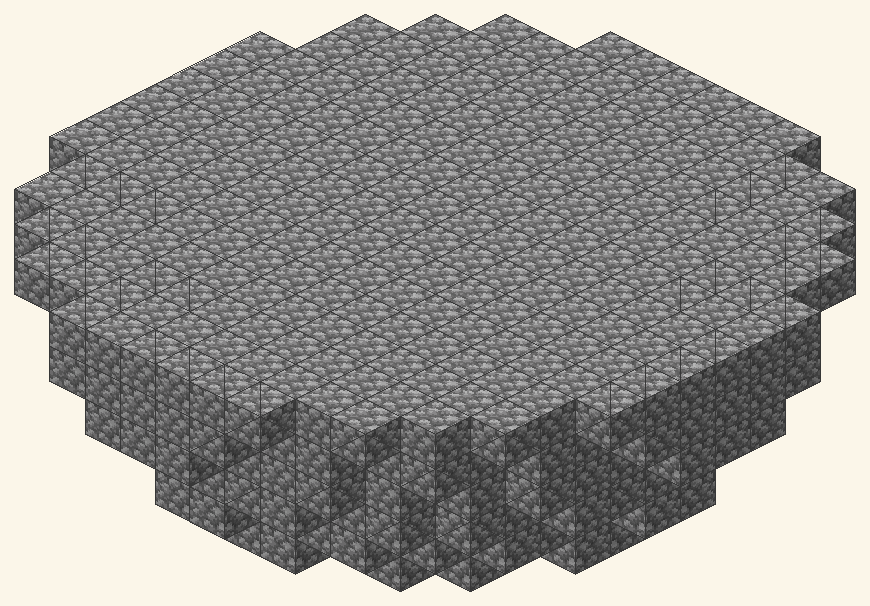
\includegraphics[width=\linewidth]{fig12_3d_cut_y50.png}
  \caption{Y 50\% 자르기 --- 고전적 \emph{돔}.}
\end{subfigure}\hfill
\begin{subfigure}[t]{0.31\linewidth}\centering
  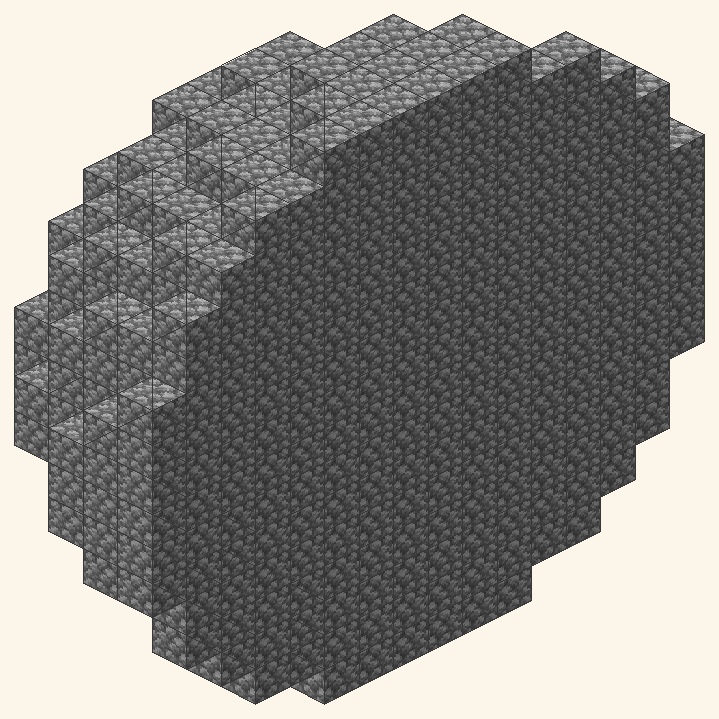
\includegraphics[width=\linewidth]{fig13_3d_cut_x50.png}
  \caption{X 50\% 자르기 --- \emph{측면 반구}.}
\end{subfigure}\hfill
\begin{subfigure}[t]{0.31\linewidth}\centering
  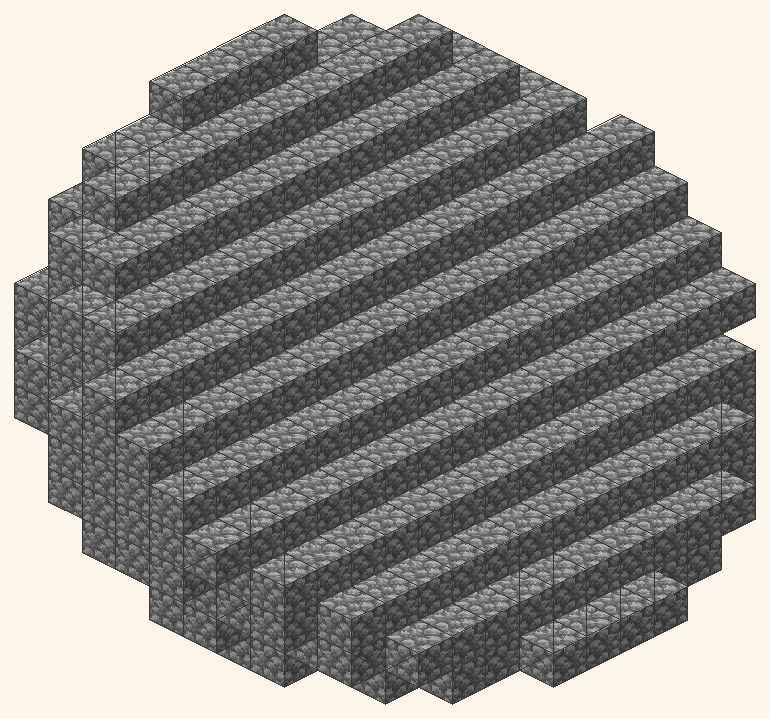
\includegraphics[width=\linewidth]{fig14_3d_cut_diag50.png}
  \caption{대각 50\% 자르기 --- \emph{비스듬한 반욕조}.}
\end{subfigure}
\caption{같은 지름 16의 타원체에 적용된 세 가지 평면 자르기, 모두 부피의 $50\%$를 보존. 대각 자르기의 특징적 계단 패턴을 살펴보세요: 두 축을 연결하는 빗변을 노출합니다. 각 자르기는 다른 마인크래프트 건축 계획: 사원 돔, 측면 반경기장, 분수의 원형극장.}
\label{fig:cortes}
\end{figure}

\begin{hwaldong}[3.4 --- 한국 시각 유산과의 대화 \quad\tempo{10분}]\label{at:34}
\emph{국어, 미술, 역사와의 연계. 본 활동은 문화 정체성과 유산에 관한 2022 개정 교육과정의 핵심 역량을 충족합니다.}

다섯 가지 이미지를 투사 (또는 인쇄 배부):

\begin{itemize}[leftmargin=1.3em,itemsep=0.2em,topsep=0.3em,nosep]
  \item \acc{첨성대} (瞻星臺, 신라 7세기, 경주): 동아시아 가장 오래된 천문대로 알려진 모듈식 화강암 구축물. 약간의 원형 곡선을 모듈로 근사한 사실상의 \emph{voxel 건축} --- 우리가 지금 공부하는 정확한 문제. \emph{석굴암 본존불} (8세기 통일신라)의 화강암 조립 반구 천장 또한 정밀한 기하학의 사례입니다.

  \item \acc{한옥 모듈식 건축}: 한옥은 \emph{칸} (間) 단위로 조립되며, 너와집 (강원도 산간), 굴피집, 초가집의 둥근 지붕, 까치구멍집 (안동) 등이 다양한 \emph{모듈 적층 voxel}을 보여 줍니다. 영주 부석사 무량수전 (12세기 고려)은 한국 最古의 모듈식 목조 건축물입니다.

  \item \acc{단청} (丹靑): 한국 건축 (사찰, 궁궐)의 채색 기하학 무늬는 직접 \emph{voxel art}와 통합니다. \acc{보자기} (褓子) — 특히 조각보 (patchwork)는 직접 \emph{voxel quilting}; \acc{화각} (花角)은 소뿔에 그린 채색 기하 문양으로 모자이크와 유사. \acc{한복 자수} (刺繡)와 \acc{색지 공예} 또한 같은 전통.

  \item \acc{빗살무늬 토기와 고인돌}: 한국 신석기 빗살무늬 토기 (5000년 전)는 voxel같은 빗금 무늬를 보여 주며, \emph{고인돌} (Dolmen — 한국에 세계에서 가장 많은 4만여 기, 강화·고창·화순 UNESCO)은 모듈식 거석 기하의 원형입니다.

  \item \acc{한국 마인크래프트 커뮤니티의 빌드}: 한국 서버, 양띵·우왁굳·풍월량의 합방 빌드, 인생게임 (Aether), 「샌드박스 네트워크」 콘텐츠 등에서 한국 청소년이 짓는 돔, 구, 아치의 타임랩스. \emph{이것이 살아 있는 한국 마인크래프트 「민족수학」} — 한국어로, 현재진행형으로, 매일.

  \item (참고) \acc{동대문 DDP} (Zaha Hadid, 2014, 서울 동대문): 매개변수 곡면 건축, 직접 voxel과 연결. \acc{롯데월드타워} (2017, 서울 송파, 555m — 한국 최고층, 윗부분 곡선). \acc{부산 누리마루 APEC 하우스} (한국 정자 + 현대 기하). \acc{인천국제공항} (거대 모듈 구조). \acc{인사동 쌈지길} (조립식 모듈 건축).
\end{itemize}

\textbf{유도 토론:} \emph{\enquote{첨성대를 만든 신라 장인은 화강암 블록으로 우리가 픽셀로 그린 같은 곡선을 만들었습니다. 빗살무늬 토기를 만든 신석기 토기장은 5000년 전에 voxel같은 패턴을 만들었습니다. 한옥의 칸 단위 건축은 1000년 전부터 본격적으로 voxel 건축이었습니다. 단청 화공은 사찰 천장에 voxel art와 똑같은 기하 무늬를 그렸습니다. 한국 마인크래프트 커뮤니티는 서버에서 매일 같은 일을 합니다. 우리가 공부하는 래스터화 문제는 디지털 시대의 발명이 아닙니다. 인간 역사의 상수입니다. 각 문화가 자신의 \emph{래스터화} 방식을 발견했습니다.}}

\textbf{학제간 연계:} 「국어」 「미술」 「역사」 「한국지리」 선생님과의 협력 권장. 4차시와 5차시는 모둠이 한국의 어떤 시각 전통에서 작업의 영감을 받을지 \emph{선택}하도록 요청합니다.

\textbf{허준이 (June Huh) 모멘트:} 활동 끝에 \acc{허준이 (June Huh, 2022 필즈상)}를 잠시 언급합니다. 한국계 미국인 수학자, 어린 시절 한국 거주, 서울대학교 졸업, KIAS (고등과학원) 연구원 출신, 프린스턴대 교수. \emph{한국 출신 최초 필즈상 수상.} 비범한 학교 성적이 아니어도 세계 최정상 수학자로 성장할 수 있다는 사례 — 한국 사교육 입시 중심 문화에 영감을 줍니다.
\end{hwaldong}

% =============================================================================
\subsection{4차시 --- \enquote{인벤토리 산술: 스택, 더블 체스트, 명령어}}\label{aula4}

\subsubsection*{차시 목표}
마인크래프트의 \emph{인벤토리 산술}을 올림 나눗셈과 몫·나머지 표현의 구체적 응용으로 소개. 핵심 명령어 (\cmd{/fill}, \cmd{/clone}, \cmd{//sphere}, \cmd{//hsphere})와 팔분 대칭 최적화 제시.

\begin{hwaldong}[4.1 --- 스택 산술 \quad\tempo{15분}]\label{at:41}
마인크래프트에서 각 인벤토리 슬롯은 \acc{같은 종류 블록 최대 64개}를 담을 수 있습니다. 이 한계가 부피 계산에 실질적 의미를 부여합니다: 구 $D=12$의 $V = 904$ 블록은 \emph{단순히 「가방에 904개」}가 아니라 \emph{\enquote{cobblestone $\lceil 904/64 \rceil = 15$ 스택 (꽉 찬 슬롯)}}을 의미합니다.

\textbf{핵심 공식:}

\begin{susik}
\centering
$\displaystyle N_{\mathrm{stacks}} = \left\lceil \dfrac{V}{64} \right\rceil
\qquad\qquad
N_{\mathrm{double\,chests}} = \left\lceil \dfrac{V}{3\,456} \right\rceil$
\end{susik}

(단상자 27 슬롯; 더블 체스트 54 슬롯; $54 \times 64 = 3\,456$ 아이템.)

\textbf{짝 활동:}
\begin{enumerate}[leftmargin=1.5em,itemsep=0.15em,topsep=0.3em,nosep]
  \item 구 $D = 8$ (부피 $\approx 268$ 블록): 스택은 몇 개? 단상자는 몇 개? 정답: 5스택; 단상자 1개 (17 슬롯 여유).
  \item 구 $D = 16$ (부피 $\approx 2\,145$ 블록): 스택은 몇 개? 더블 체스트는 몇 개? 정답: 34스택; 더블 체스트 1개 (20스택 더 들어감 — 작은 원기둥 하나 더 만들 여유).
  \item 구 $D = 32$ (부피 $\approx 17\,156$ 블록): 스택은 몇 개? 더블 체스트는 몇 개? 정답: 269스택 ($\approx$ 더블 체스트 5개 + 1스택), $\lceil 17\,156/3\,456 \rceil = 5$ 더블 체스트.
  \item \emph{마인크래프트에서, 서바이벌 모드 한국 광부는 곡괭이 등급에 따라 cobblestone 1스택을 4--6분에 추출합니다. 구 $D = 16$의 총 채집 시간 추정: $34 \times 5 = 170$분 $\approx 2{,}8$시간.}
\end{enumerate}
\end{hwaldong}

\begin{hwaldong}[4.2 --- 마인크래프트 명령어 \quad\tempo{15분}]\label{at:42}
핵심 명령어 제시:

\begin{itemize}[leftmargin=1.4em,itemsep=0.25em,topsep=0.3em]
  \item \cmd{/setblock x y z minecraft:stone} --- 특정 위치에 블록 배치.
  \item \cmd{/fill x1 y1 z1 x2 y2 z2 minecraft:stone} --- 직사각형 박스를 블록으로 채움. 바닐라 한계: 명령당 $32\,768$ 블록.
  \item \cmd{/clone x1 y1 z1 x2 y2 z2 x3 y3 z3} --- 영역을 다른 위치로 복사 (대칭 건축의 기본 도구).
  \item \cmd{//sphere stone 8} (WorldEdit) --- 플레이어 중심에 반지름 8의 구 작도, 브레젠험 3D 알고리즘 사용.
  \item \cmd{//hsphere stone 8} (WorldEdit) --- 속 \emph{빈} 구 (껍질만). 내부가 비어 있는 돔에 유용.
  \item \cmd{//ellipsoid stone 10 5 10} (WorldEdit) --- $W = 20, H = 10, D = 20$의 타원체, 지정된 반축.
\end{itemize}

\textbf{시연 (마인크래프트가 가능하면):} 테스트 월드에서 \cmd{//sphere stone 8} 실행 후 측정. Block Round에서 지름 16의 브레젠험 결과와 비교. 두 출력의 수학적 동일성 확인.

\textbf{마인크래프트가 없는 경우:} 정신적으로 실행. 모눈종이에 메모: \enquote{나는 땅 (y=64)에 서 있고, 땅에서 8블록 위 (y=72)부터 반지름 8의 구를 만들고 싶다. 어떤 명령어?} 정답: $(0, 72, 0)$에서 \cmd{//sphere stone 8}.
\end{hwaldong}

\begin{hwaldong}[4.3 --- 팔분 대칭 최적화 \quad\tempo{15분}]\label{at:43}
\textbf{핵심 아이디어:} 원점 중심의 구는 세 좌표평면에서의 반사에 대해 불변. 군 $\mathbb{Z}_2^3$은 위수 8: 한 \emph{팔분원} (영역 $+x, +y, +z$)에서 시작하면 나머지 일곱 영역은 반사로 얻어집니다.

\textbf{실용적 함의:} $V$개 블록을 하나씩 놓는 대신, 양의 팔분원에 $V/8$ 블록을 만들고 \cmd{/clone}으로 7번 반사.

\begin{susik}
\centering
$\displaystyle \mathrm{cost}_\mathrm{symmetry} = N_\mathrm{octant} + 7\, T_\mathrm{clone}
\;\ll\; \mathrm{cost}_\mathrm{brute-force} = N\, T_\mathrm{block}$
\end{susik}

\textbf{구체적 예시, $(0, 72, 0)$ 중심의 $D = 24$ 구:}
\begin{enumerate}[leftmargin=1.5em,itemsep=0.15em,topsep=0.3em,nosep]
  \item 양의 팔분원을 수동으로 구축 ($\approx 905$ 블록, 서바이벌에서 $\approx 15$분 또는 크리에이티브 브러시로 $\approx 45$초).
  \item $-x$ 반사: \cmd{/clone 0 72 0 12 84 12 -12 72 0 mode:masked}
  \item $-y$ 반사: \cmd{/clone 0 72 0 12 84 12 0 60 0 mode:masked}
  \item $-z$ 반사: \cmd{/clone 0 72 0 12 84 12 0 72 -12 mode:masked}
  \item 팔분원 $(-x, -y)$, $(-y, -z)$, $(-x, -z)$, $(-x, -y, -z)$: 유사 명령어.
\end{enumerate}

\textbf{시간 비교:}
\begin{itemize}[leftmargin=1.3em,itemsep=0.1em,topsep=0.2em,nosep]
  \item 대칭 없이 서바이벌: $7\,238$ 블록 $\times$ 2초/블록 $\approx$ 4시간.
  \item 대칭으로: 15분 (팔분원) + 0.5초 (7클론) $\approx$ 15분.
  \item 가속: \emph{16배}.
\end{itemize}
\end{hwaldong}

\begin{hwaldong}[4.4 --- 응용: 실제 돔 계획 \quad\tempo{5분}]
짝으로, \emph{종이나 Block Round에서} 첨성대 양식의 천문대, 한옥 기와지붕을 모티프로 한 사원, 단청 무늬 신전 위에 Quartz $D=20$ 돔 건축을 계획. 메모:
\begin{itemize}[leftmargin=1.3em,itemsep=0.1em,topsep=0.2em,nosep]
  \item 돔 부피 (구 $D=20$의 절반): $\approx 2\,094$ 블록.
  \item 필요 스택: 33스택.
  \item Quartz block 수 (각 1개당 Nether Quartz 4개 필요, Nether에서 채굴 가능): $\sim 2\,094 \times 4 = 8\,376$ Nether Quartz.
  \item 대칭을 활용한 최적 명령어 시퀀스.
\end{itemize}

이 활동은 5차시 (실제 건축)의 토대를 마련합니다.
\end{hwaldong}

% =============================================================================
\subsection{5차시 --- \enquote{실제 건축: Block Round에서 마인크래프트로}}\label{aula5}

\subsubsection*{차시 목표}
모든 학습 내용을 \emph{자작 건축 산물}로 동원: Block Round에서 출력, 마인크래프트로 임포트 (Litematica 또는 Schematica 사용), 크리에이티브 또는 서바이벌에서 건축. 수학적 선택 옹호와 최종 산출물 제출을 통해 학습 평가.

\begin{hwaldong}[5.1 --- 도전 과제 발표 \quad\tempo{5분}]\label{at:51}
\textbf{지시:} \emph{\enquote{짝 또는 모둠으로, Block Round에서 생성된 도형 (원, 타원, 구, 타원체) 최소 세 개를 결합한 마인크래프트 (또는 마인크래프트가 없으면 Block Round) 건축물을 만드세요. 학급 서버의 도시, 사원, 둥근 농장, 천문대 — 여러분이 선택. 각 모둠은 작품을 발표하고 \acc{수학적으로} 선택을 설명: 왜 이 알고리즘? 왜 이 비율? 왜 이 자르기? 왜 이 블록?}}
\end{hwaldong}

\begin{hwaldong}[5.2 --- 내보내기와 들여오기 \quad\tempo{15분}]\label{at:52}
Block Round $\rightarrow$ 마인크래프트 흐름 시연:

\begin{enumerate}[leftmargin=1.5em,itemsep=0.2em,topsep=0.3em]
  \item Block Round에서 원하는 도형 설정 (예: Y 50\% 자르기의 Quartz 구 $D = 12$).
  \item 캔버스 모서리의 \emph{Export Schematic} 버튼 클릭. \texttt{.schem} 파일 (Sponge Schematic v2) 다운로드.
  \item 마인크래프트 자바 에디션 + \emph{Litematica} 모드 (무료) 설치: 모드 열고, \emph{Load Schematic}, 다운로드한 파일 선택.
  \item Litematica가 플레이어가 선택한 위치에 건축의 반투명 \enquote{유령}을 표시.
  \item 플레이어가 각 블록을 \emph{유령을 따라} 배치. Litematica는 잘못된 블록을 빨강으로 강조.
  \item \emph{\cmd{//schem load} 대안:} WorldEdit이 있는 서버에서 \cmd{//schem load file\_name}로 임포트, \cmd{//paste -a}로 현재 위치에 붙여넣기 --- 즉시 건축.
\end{enumerate}

\textbf{마인크래프트가 없으면:} \texttt{.schem} 내보내기를 시연하고 16진 편집기로 바이너리 파일 표시 --- Sponge v2, gzip, NBT 포맷 토론. 정보과 통합과정 활동.
\end{hwaldong}

\begin{hwaldong}[5.3 --- 제작 \quad\tempo{20분}]\label{at:53}
\textbf{모둠당 준비물:}
\begin{itemize}[leftmargin=1.3em,itemsep=0.15em,topsep=0.3em,nosep]
  \item Block Round 접근 (컴퓨터 또는 \emph{스마트폰});
  \item (선택) Litematica 또는 Schematica가 있는 마인크래프트 접근;
  \item 스케치와 시나리오 작성용 모눈종이, 연필, 사인펜;
  \item 세 개 의무 질문이 있는 시나리오 시트 (부록~\ref{ap:exerc}, 연습 8).
\end{itemize}

\textbf{모둠 작업 내부 단계:}
\begin{enumerate}[leftmargin=1.5em,itemsep=0.15em,topsep=0.3em,nosep]
  \item \tempo{5분} 브레인스토밍과 종이 스케치.
  \item \tempo{8분} Block Round에서 제작과 \texttt{.schem} 내보내기.
  \item \tempo{5분} 마인크래프트에서 임포트와 빠른 테스트 (가능 시).
  \item \tempo{2분} 시나리오에 수학적 정당화 서술.
\end{enumerate}

\textbf{교사 순회:} 모둠 사이를 돌며 매개 질문 --- \emph{\enquote{왜 이 알고리즘을 선택했나요? 이 자르기를 부등식으로 어떻게 표현할 수 있나요? Quartz 더블 체스트가 몇 개 필요한가요?}}
\end{hwaldong}

\begin{hwaldong}[5.4 --- 발표와 집단 종합 \quad\tempo{10분}]\label{at:54}
각 모둠은 2분 동안 작품을 학급에 발표, 프로젝터 (또는 마인크래프트, 또는 종이 작품)로 보여 주고 세 가지 수학 질문 중 \emph{최소 하나}에 답합니다.

\textbf{발표의 최소 기준:}
\begin{itemize}[leftmargin=1.3em,itemsep=0.1em,topsep=0.2em,nosep]
  \item 존재하는 수학 도형 최소 하나 식별;
  \item 선택한 알고리즘 명명, 의도한 시각적 효과에 적합한 이유 정당화 (사후적이라도);
  \item 3D 자르기가 있다면 부등식으로 기술;
  \item 필요한 스택/더블 체스트 수 추정 (대략이라도).
\end{itemize}

\textbf{교사의 최종 종합 (3분):} 시퀀스의 중심 아이디어 회복 --- \emph{\enquote{이산 복셀 격자에서, 같은 연속 곡면은 다중 표현을 허용합니다; 하나를 선택하는 것은 수학적 결정입니다; 그것을 마인크래프트에 짓는 것은 시민의식, 자원 관리, 미학의 결정입니다}} --- 그리고 한국 현대 수학의 지평에 위치 짓기: 학급에 \hyperref[sec:olympiad]{KMO}와 \hyperref[sec:olympiad]{KOI} 탐색, 허준이의 사례와 KIAS·POSTECH·서울대·KAIST 수학의 길 안내, 한국 마인크래프트 협동 서버에서 더 큰 건축에 도전할 것을 권합니다.
\end{hwaldong}

\begin{minecraft}[확장 가능성]
5차시는 여러 교과외 프로젝트 확장 가능성을 엽니다:
\begin{itemize}[leftmargin=1.3em,itemsep=0.15em,topsep=0.3em,nosep]
  \item \textbf{수학 도시 프로젝트:} 학급이 학교 서버에서 도시를 짓되 각 건물은 기하 도형 (원기둥, 구, 타원체, 이차곡선 조합)을 구현.
  \item \textbf{한국 문화유산 재현:} 마인크래프트에서 첨성대, 석굴암 본존불 천장, 부석사 무량수전, 동대문 DDP, 롯데월드타워, 한옥 (수원화성도!)을 voxel로 재구성.
  \item \textbf{Block Round 올림픽:} 학급 내 경쟁 --- 연속 부피에 가장 가까운 구를 짓는 모둠? 대칭 활용으로 가장 시간을 단축하는 모둠?
  \item \textbf{마이스터고·특성화고와의 연계:} Block Round를 사전-공학 샌드박스로 활용: 측지선 돔, 복셀화 트러스, 평탄 곡면을 근사하는 구조물. 게임 콘텐츠 마이스터고 학생에게 직접 연결.
  \item \textbf{KOI/정보과와의 연계:} 세 알고리즘을 Python 또는 Scratch로 재구현, Block Round 결과와 비교, 학생부 종합 전형 탐구 활동으로 제출.
\end{itemize}
\end{minecraft}

% =============================================================================
\section{평가}\label{sec:avaliacao}

평가는 \acc{형성 평가}, \acc{과정 평가}, \acc{총괄 평가} 모델을 채택하며, 네 차원 (마인크래프트 적용에 특화된 다섯 번째 차원 포함)을 통합합니다. 한국교육과정평가원 (KICE)의 「과정 중심 평가」 정책과 학생부 종합 전형의 정성 평가 전통에 부합합니다.

\subsection{진단 평가}
1차시, 활동 1.2 (원의 수동 작도)에서 실시. 교사가 좌표평면, 원의 방정식, 셈하기의 어려움을 식별 --- 코로나19 이후 「과정 중심 평가」 결과에서 드러난 결손을 보완.

\subsection{형성 평가}
다섯 차시에 분산: 참여 직접 관찰, \emph{think--pair--share}에서의 응답 품질, 활동~\ref{at:25}, \ref{at:32}, \ref{at:41}의 계산에 대한 \emph{즉각} 피드백.

\subsection{총괄 평가}
두 가지 제출로 구성:

\begin{enumerate}[leftmargin=1.5em,itemsep=0.2em,topsep=0.3em,nosep]
  \item \textbf{연습 문제집} (부록~\ref{ap:exerc}), 8문항, 5차시 끝 또는 합의된 날짜에 제출.
  \item \textbf{최종 프로젝트} (활동~\ref{at:53}), 발표 시 시나리오 응답 (활동~\ref{at:54}).
\end{enumerate}

\subsection{평가 루브릭}

\begin{center}
\small
\begin{tabularx}{\textwidth}{@{}p{0.21\textwidth}XX@{}}
\toprule
\textbf{차원} & \textbf{충분히 만족 (8--10)} & \textbf{부분 만족 (5--7) / 불충분 (0--4)} \\
\midrule
\textbf{수학 개념} & 타원/타원체의 음함수 방정식을 정확히 적용; 세 알고리즘 기준과 차이 인식. & 원의 기본 방정식은 적용하나 타원 일반화 혼동 / 알고리즘 차이 인식 못 함. \\
\addlinespace[3pt]
\textbf{소프트웨어 활용 (Block Round)} & 2D와 3D에서 Block Round를 자율적으로 조작; 이미지와 \texttt{.schem} 출력; 알고리즘과 스타일 전환. & 잦은 보조 필요; 2D만 조작. \\
\addlinespace[3pt]
\textbf{주장} & 최종 프로젝트의 선택을 수학적으로 정당화; 적절한 전문 어휘 사용 (\emph{알고리즘}, \emph{복셀}, \emph{자르기}, \emph{부등식}, \emph{스택}, \emph{더블 체스트}). & 수학 동원 없이 미적으로만 정당화; 어휘 부재. \\
\addlinespace[3pt]
\textbf{마인크래프트 실용 적용} & 프로젝트의 스택과 더블 체스트를 정확히 계산; \cmd{/fill} 또는 \cmd{//sphere} 명령 시퀀스 기술; 팔분 대칭 활용. & 몫과 나머지 혼동; 블록을 단독 단위로 취급; 대칭 미사용. \\
\addlinespace[3pt]
\textbf{협력} & 짝/모둠에서 생산적 작업; 집단 토론에 기여. & 단독 작업; 기여 적음. \\
\bottomrule
\end{tabularx}
\end{center}

\subsection{성적 환산}
\begin{itemize}[leftmargin=1.3em,itemsep=0.1em,topsep=0.2em,nosep]
  \item 연습 문제집: 평가의 40\%.
  \item 최종 프로젝트 + 발표: 평가의 50\%.
  \item 과정 관찰 (참여): 평가의 10\%.
\end{itemize}

\subsection{학생부 종합 전형과의 연결}

본 수업의 결과물 (5차시 자작 작품, 연습 문제집, 발표 영상)은 \acc{학생부 종합 전형}의 \emph{탐구 활동}, \emph{진로 활동}, \emph{자율 활동}으로 학교생활기록부에 기재할 수 있습니다. 특히 마이스터고·특성화고 학생에게는 \emph{전공 관련 탐구}로, 일반고 학생에게는 \emph{수학·정보 융합 탐구}로 의미 있는 자료가 됩니다.

% =============================================================================
\section{한국 수학·정보 교육 생태계와의 연계}\label{sec:olympiad}

본 시퀀스는 한국 수학·정보 교육과 연구의 \emph{풍부한 생태계} 안에 위치하며, 교사가 확장·심화 자료로 활용할 수 있습니다.

\subsection{KMO --- 한국수학올림피아드}

\acc{대한수학회 (KMS, Korean Mathematical Society)}가 주관하는 \href{https://www.kmo.or.kr/}{한국수학올림피아드 (KMO)}는 한국의 대표적 수학 경시대회입니다. 한국주니어수학올림피아드 (KJMO)는 중학생 대상이며, KMO 우수자는 아시아·태평양 수학올림피아드 (APMO Korea)와 국제수학올림피아드 (IMO) 한국 대표로 선발됩니다.

\emph{본 시퀀스의 내용 (원과 타원체의 해석기하, 알고리즘 추론, 수치 근사)은 KMO 2차 시험과 IMO 기하 영역에 직접 준비 자료가 됩니다.}

\subsection{KOI --- 한국정보올림피아드}

\href{https://www.digitalculture.or.kr/koi/}{한국정보올림피아드 (KOI)}는 한국정보화진흥원 (NIA)이 주관하며 국제정보올림피아드 (IOI) 한국 대표를 선발합니다. KOI 지역 예선은 전통적으로 브레젠험 같은 고전 알고리즘을 출제 주제로 포함합니다 (활동~\ref{at:23}에서 다룸). 한국컴퓨터과학경시대회와 알고리즘 챔피언십도 본 수업과 연계 가능.

\subsection{영재교육 시스템}

한국의 영재교육 시스템은 \emph{영재학교} (전국 8개교: 한국과학영재학교 KSA, 서울과학고, 경기과학고, 대구과학고, 광주과학고, 인천과학예술영재학교, 대전과학고, 세종과학예술영재학교) + \emph{과학고등학교} (전국 20여 개교) + \emph{대학부설 영재교육원} + \emph{교육청 영재교육원}으로 구성됩니다. 한국수학회 산하 영재교육원도 운영됩니다. 본 시퀀스에서 5차시 최종 프로젝트로 두각을 보이는 학생은 영재교육원 추천이나 대학부설 R\&E (Research \& Education) 프로그램 참여를 추천할 수 있습니다.

\subsection{허준이 (June Huh)와 한국 수학의 자존감}

2022년, \acc{허준이} (June Huh)는 \emph{한국 출신 최초로 필즈상을 수상}했습니다 --- 수학계 최고의 영예. 한국계 미국인이며, 어린 시절 한국 거주, 서울대학교 졸업, KIAS (고등과학원) 박사후 연구원, 현재 프린스턴대 교수. 그는 한국 사교육 입시 위주 문화에서 비범한 학교 성적을 보이지 않았던 학생이 어떻게 세계 최정상 수학자가 될 수 있는지에 대한 상징적 사례로 한국 수학계의 자존감과 가능성을 대표합니다.

다른 한국 출신·한국계 수학자: \acc{이임학} (Lee Im-hak, 1922--2005, 한국 현대 수학의 개척자, 캐나다 브리티시컬럼비아 대학; 한국에서 미국·캐나다로의 두뇌유출의 상징); \acc{김민형} (Minhyong Kim, 영국 옥스퍼드대 + 미국 워릭대 + 한국 KIAS, 산술 기하학; 「수학자의 시선으로」 저자); \acc{박형주} (Hyungju Park, POSTECH/연세대, 2014 ICM 서울 조직위원장 --- 한국에서 처음 열린 ICM!).

\subsection{한국 수학 연구 기관}

\href{http://www.kias.re.kr/}{고등과학원 (KIAS, Korea Institute for Advanced Study --- 1996 설립, 서울 동대문구)}는 한국 이론 수학 연구의 메카입니다. \href{http://www.nims.re.kr/}{국가수리과학연구소 (NIMS, National Institute for Mathematical Sciences --- 대전)}, \href{https://www.ibs.re.kr/}{기초과학연구원 (IBS --- 수학 관련 연구단)}, KAIST 수리과학과, POSTECH 수학과, 서울대 자연과학대 수리과학부, 연세대·고려대 수학과 등이 한국 수학 연구의 중심을 이룹니다.

\subsection{마인크래프트 에듀케이션 에디션 (한국 마이크로소프트 + 교육부 협력)}\label{sec:mee}

\emph{마인크래프트 에듀케이션 에디션}은 학교에서 무상 이용 가능한 교육용 변형입니다 (Microsoft 365 Education A1/A3 라이센스로 제공). 한국 마이크로소프트와 교육부의 협력으로 일부 시·도 교육청에서 「디지털 새싹 교실」 사업의 일환으로 시범 운영됩니다. 「샌드박스 네트워크」 등 한국 콘텐츠 회사가 관련 교육 영상을 제작합니다. \emph{본 시퀀스는 호환 가능}: Block Round가 내보내는 \texttt{.schem}은 자바 에디션 (Litematica 경유)으로 임포트 가능하며, 에듀케이션 에디션용으로도 cmdblocks를 통해 우회 임포트 가능.

\subsection{한국 마인크래프트 커뮤니티와 voxel 아키텍처}

한국 마인크래프트 커뮤니티는 \emph{레드스톤 엔지니어링} (게임 내 회로로 구현된 논리 컴퓨팅 --- 실제 디지털 회로 등가)과 \emph{대형 건축}에 특화된 채널이 활발합니다. 양띵, 우왁굳, 풍월량, 침착맨 (이병건), 인생게임 (Aether), 자나깨나, 김메주와 고양이들, 「샌드박스 네트워크」 콘텐츠 등이 교사가 맥락화에 활용할 수 있는 문화 참조입니다. 한국 서버 (와치 마크 Lunarcraft, mc.frwby.kr 등). \emph{보충 활동:} 학생들에게 한국어 튜토리얼 링크를 가져오고 그 안의 암시적 수학을 분석하도록 요청.

\subsection{민족수학과 자기주도학습}

한국 수학교육에서 민족수학 (D'Ambrosio 한국어 번역본 있음)과 \emph{자기주도학습} (셀프-디렉티드 러닝)은 깊이 연결됩니다. 한국 민족수학 연구자: 한대희, 송상헌 등. 한국 사교육 문화에서 강조되는 자기주도학습은 Block Round의 탐구·발견 접근에 직접 부합합니다.

\subsection{교원 양성과 PROFMAT 등가}

한국에서 수학 교사가 되려면 \acc{교원자격검정}을 거쳐 교원자격증 (수학과 정교사 2급)을 취득해야 합니다. 사범대학 (서울대 사범대, 한국교원대 등), 일반대학 교직과정, 또는 교육대학원 (수학교육 전공) 경로를 통합니다. 본 시퀀스는 교육대학원 석사 학위 논문 (학위 청구 작품)의 기반이 될 수 있으며, 한국수학교육학회와 대한수학교육학회 연구 논문 (수학교육 학회지)으로 출판할 수 있습니다.

% =============================================================================
\section{학제간 연계}\label{sec:interdisc}

\subsection{미술·국어와의 연계}
\emph{복셀 아트}는 전통적으로 미술 언어로 다뤄집니다. Block Round는 수학과 미술을 같은 대상에서 결합하는 드문 기회를 제공: 도형은 \emph{동시에} 방정식이며 미적 구성입니다. \emph{한국 단색화} (Dansaekhwa --- 박서보, 정상화, 이우환, 윤형근의 단순 기하 + 격자, 직접 voxel art!), 김환기의 \emph{「점」 시리즈} (1970년대 --- 픽셀/voxel 같은 추상), \emph{한국 민화} (民畵 --- 기하학적 십장생, 화조도 패턴), \emph{보자기 조각보} (직접 voxel quilting), \emph{단청} (한국 건축의 채색 기하)와의 깊은 연결. \acc{백남준} (Nam June Paik, 1932--2006, 비디오 아트의 아버지, 韓國系 --- 디지털 아트의 기원!)은 한국이 디지털 아트 세계에 끼친 영향을 상징합니다. 미술 교사와의 협력으로 학교 게시판 또는 SNS에서 최종 작품 전시 권장.

\subsection{물리·정보와의 연계}
Block Round의 소리 레이어는 사인파의 가산 합성을 사용합니다 (Pixel Round와 유사). 선택된 주파수는 \acc{12평균율}의 음에 근사합니다 (각 반음은 주파수를 $2^{1/12} \approx 1{,}0595$배). 흥미롭게도 \emph{조선 시대 박연 (朴堧)이 1419년에 「악학궤범」 9년 전} 12평균율 이론을 정리했으며 --- 이는 조선 음악 이론과 음높이 수학의 깊은 한국 전통입니다. 마인크래프트에서는 \emph{레드스톤} (디지털 논리 = 부울 대수 = 섀넌 정보 이론), \emph{음표 블록}, \emph{물리 시뮬레이션} (모래 낙하, 물 흐름)과 연계. 한국 정보과학자 (이수영 KAIST 등)의 연구도 참고.

\subsection{「정보과」와의 연계 (2022 개정 교육과정 정보과 강화)}
브레젠험 알고리즘은 컴퓨터 과학의 고전입니다. \emph{컴퓨팅 사고} 수업과 연계: \emph{추상화} (방정식이 모델), \emph{분해} (도형이 복셀 집합), \emph{패턴 인식} (대칭), \emph{알고리즘화} (세 절차). \hyperref[sec:olympiad]{KOI}와 「인공지능 수학」 「정보과」 진로선택과의 직접 연결. \texttt{.schem} 생성 (Sponge v2 + gzip + NBT)은 바이너리 직렬화의 \emph{사례 연구} --- 마이스터고 (SW·게임·반도체) 통합과정과 직결.

\subsection{역사·한국지리와의 연계}
Bresenham은 1965년 미국 IBM에서 알고리즘을 발표했습니다. 같은 시기 한국 컴퓨팅의 첫걸음: KIST 한국과학기술원의 IBM 1401 (1967), 서울대 IBM 1401 (1968). \emph{삼성전자} (1969 설립)는 현재 세계 최대 메모리 반도체 제조사로 voxel 아트의 \emph{물리적 기반} (반도체!)을 만듭니다. 게임 산업: 넥슨 (1994), 엔씨소프트 (1997), 크래프톤 (배틀그라운드), 펄어비스 (검은사막) --- 한국 게임 산업은 voxel/픽셀 아트의 글로벌 강국. 비교 연대표: \emph{세종대왕 한글 1443 / 박연 12평균율 1419 / 첨성대 7세기 / 정약용 18세기 / Bresenham 1965 / 삼성전자 1969 / 넥슨 1994 / Markus Persson 2009}. K-Pop & 한류 (Hallyu): BTS, BLACKPINK, 「오징어 게임」 --- 한국 디지털 문화의 세계화. 한국이 세계 반도체 시장의 약 50\%를 공급한다는 사실은 \emph{글로벌 voxel art의 인프라를 한국이 만든다}는 의미입니다.

\subsection{한국지리·환경과의 연계}
래스터화는 \emph{복셀 아트}만의 주제가 아닙니다: \emph{지리정보시스템 (GIS)}의 기초입니다. 디지털 지도, 위성 영상 (한국항공우주연구원 KARI의 아리랑 위성), \href{http://www.nsdi.go.kr/}{국토교통부 국가공간정보포털}, KMA 기상청 격자 데이터 (직접 voxel!), \emph{디지털 트윈 서울} (Seoul Digital Twin --- 거대 voxel 도시 모델!)은 본 시퀀스가 다루는 수학 문제와 같은 현대 한국 사례입니다.

\subsection{공학과의 연계 (마이스터고·특성화고 통합과정)}
마인크래프트는 마이스터고와 특성화고에서 사전-공학 샌드박스로 \emph{현저히} 활용됩니다: 학생은 도시 시뮬레이션, 레드스톤 회로 전기 시스템, 물의 유압 시스템, 피스톤 기계 시스템을 구현. 본 시퀀스의 복셀 기하는 \emph{기계 공학}, \emph{재료 역학}, \emph{구조 공학} 입문자에게 필수 수학입니다. 한국 공과대학 (KAIST, POSTECH, 서울대, 연세대, 고려대, 한양대)과 마이스터고 (SW, 반도체, 게임, 자동차 분야), 4차 산업혁명 정책의 메이커스페이스·무한상상실에서의 활용도 가능합니다. \emph{한국공학교육인증} (ABEEK) 인증을 받은 공대 진학을 목표로 하는 학생에게 좋은 도전 과제.

% =============================================================================
\section{참고문헌}\label{sec:referencias}

\subsection{한국 수학교육과 교육학}
\begin{itemize}[leftmargin=1.3em,itemsep=0.15em,topsep=0.3em]
  \item 김기석 \emph{한국 교육과정 연구의 토대}. 서울: 한국교육학회, 다년도.
  \item 김정환 \emph{전인교육의 이론과 실제}. 서울: 한국교육철학회, 다년도.
  \item 신선우, 박만구, 황선욱 \emph{학교수학교육론}. 서울: 한국수학교육학회.
  \item 박교식 \emph{인지 발달과 수학 학습}. 서울대 사범대.
  \item 정영근 \emph{수학교육학 개론}. 서울대 사범대.
  \item 강성균, 송수환 \emph{수학교육 연구}. 다년도.
  \item 한대희, 송상헌 \emph{민족수학과 한국 수학교육}. 다년도.
  \item 율곡 이이 \emph{격몽요결} (擊蒙要訣, 1577). 자기주도학습의 동아시아 전통.
  \item 정약용 \emph{여유당전서} (與猶堂全書). 조선 후기 실학과 수학.
\end{itemize}

\subsection{국제 수학교육 (한국어 번역본 활용 가능)}
\begin{itemize}[leftmargin=1.3em,itemsep=0.15em,topsep=0.3em]
  \item Vygotsky, L. S. \emph{사고와 언어} (\emph{Pensamento e Linguagem}, 1934). 한국어 번역본.
  \item Bruner, J. \emph{발견 학습의 모형} (\emph{The Process of Education}, 1960). 한국 수학 교과서 (2015·2022 개정)에 깊은 영향.
  \item Polya, G. \emph{어떻게 풀까} (\emph{How to Solve It}, 1945). 한국어 번역본.
  \item Lakatos, I. \emph{증명과 반증} (\emph{Proofs and Refutations}, 1976). 한국어 번역본.
  \item D'Ambrosio, U. \emph{민족수학} (\emph{Etnomatemática}, 한국어 번역본).
  \item Skovsmose, O. \emph{비판적 수학교육} (\emph{Towards a Philosophy of Critical Mathematics Education}). 한국어 번역본.
\end{itemize}

\subsection{게임·마인크래프트와 한국 교육 연구}
\begin{itemize}[leftmargin=1.3em,itemsep=0.15em,topsep=0.3em]
  \item 한국교육학술정보원 (KERIS) \emph{디지털 교육 보고서}. 다년도.
  \item 한국교육개발원 (KEDI) \emph{교육 통계}. 다년도.
  \item Microsoft 한국 \emph{마인크래프트 에듀케이션 에디션 한국 포털}. \url{https://education.minecraft.net/ko-kr}.
  \item 교육부 \emph{2022 개정 초·중등 교육과정 총론}. 교육부 고시 제2022-33호.
  \item 한국정보화진흥원 (NIA) \emph{청소년 인터넷 이용실태조사}. 다년도.
  \item OECD PISA \emph{한국 수학 결과}. 다년도.
\end{itemize}

\subsection{공식 문서와 법령}
\begin{itemize}[leftmargin=1.3em,itemsep=0.15em,topsep=0.3em]
  \item 교육부 \emph{2022 개정 초·중등 교육과정} (교육부 고시 제2022-33호, 2024년부터 단계적 시행).
  \item 대한민국 \emph{교육기본법}, \emph{초·중등 교육법}. 법제처.
  \item 대한민국 \href{https://www.law.go.kr/}{\emph{개인정보 보호법 (PIPA)}} (2011년 제정, 2023년 개정).
  \item 대한민국 \emph{정보통신망 이용촉진 및 정보보호 등에 관한 법률} (정보통신망법).
  \item 대한민국 \emph{청소년 보호법}.
  \item 한국교육과정평가원 (KICE) \emph{대학수학능력시험 출제 자료}. \url{https://www.kice.re.kr/}.
\end{itemize}

\subsection{기술 참고문헌}
\begin{itemize}[leftmargin=1.3em,itemsep=0.15em,topsep=0.3em]
  \item BRESENHAM, J. E. Algorithm for computer control of a digital plotter. \emph{IBM Systems Journal}, v. 4, n. 1, p.~25--30, 1965.
  \item PITTEWAY, M. L. V. Algorithm for drawing ellipses or hyperbolae with a digital plotter. \emph{The Computer Journal}, v. 10, n. 3, p.~282--289, 1967.
  \item Sponge Schematic specification v2, \url{https://github.com/SpongePowered/Schematic-Specification}.
  \item WorldEdit documentation, \url{https://worldedit.enginehub.org}.
  \item Block Round --- 한국어 기술 문서: \texttt{docs\_math/Block\_Round\_Math\_ko-KR.pdf}.
\end{itemize}

\subsection{한국 수학 관련}
\begin{itemize}[leftmargin=1.3em,itemsep=0.15em,topsep=0.3em]
  \item 김민형 \emph{수학자의 시선으로}. 서울: 다산북스.
  \item 대한수학회 (KMS) \emph{수학동아} 등 다양한 잡지. \url{https://www.kms.or.kr/}.
  \item KMO \emph{한국수학올림피아드 기출문제 모음}. \url{https://www.kmo.or.kr/}.
  \item KIAS 고등과학원 \emph{대중강연 자료}. \url{http://www.kias.re.kr/}.
  \item 정약용 \emph{여유당전서} 「기하원본 한역」. 조선 시대 한국 수학사.
\end{itemize}

\newpage
% =============================================================================
% 부록
% =============================================================================
\appendix
\renewcommand{\thesection}{\Alph{section}}
\setcounter{section}{0}

\section{Block Round 라이브 시연 시나리오}\label{ap:roteiro}

초기 시연 (활동 1.3)과 교사 친숙화를 위한 권장 시퀀스. 총 시간: 15분.

\subsection{시작과 2D 모드}
\begin{enumerate}[leftmargin=1.5em,itemsep=0.15em,topsep=0.3em]
  \item Block Round 열기 (\url{https://vinisouza128.github.io/block-round/}). 학급과 함께 보이는 요소 관찰: 상단 막대, 중앙 그리기 영역 (\emph{canvas}), 측면 컨트롤, 아래의 블록 선택기.
  \item 모드가 \acc{2D / Circle}인지 확인.
  \item \emph{Size} 슬라이더를 10으로 조정. 도형 관찰 (본 지도안의 그림~\ref{fig:comp-d10}~(a)와 비교).
  \item 캔버스 하단 모서리에서 \emph{Info chip} 버튼 작동. 학급이 큰 소리로 읽기: \enquote{Diameter 10, Radius 5, Blocks $\dots$, Algorithm Euclidean}.
  \item \acc{Euclidean} / \acc{Bresenham} / \acc{Threshold} \emph{pills}를 클릭하며 세 알고리즘 사이를 전환. 각각 30초씩 멈춤.
\end{enumerate}

\subsection{블록 텍스처}

\begin{enumerate}[leftmargin=1.5em,itemsep=0.15em,topsep=0.3em]
  \item 지름 10과 유클리드 알고리즘 유지.
  \item 블록 교체 시연: \emph{Cobblestone}, \emph{Oak Planks}, \emph{Quartz Block}, \emph{Diamond} 순. 형태가 \emph{변하지 않음}, 텍스처만 변함을 관찰.
  \item 토론: \emph{\enquote{같은 구를 보고 계십니다 --- 수학은 동일합니다. 옷만 바뀌었습니다. 마인크래프트에서는 블록을 선택하고, 여기서는 시각화를 위한 텍스처만 선택합니다.}}
\end{enumerate}

\needspace{18\baselineskip}
\subsection{타원}

\begin{figure}[!htbp]
\centering
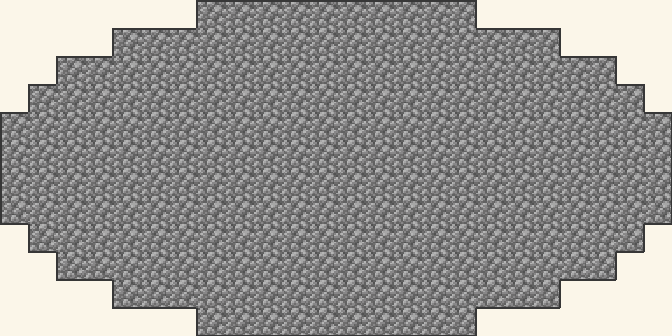
\includegraphics[width=0.45\textwidth]{fig07_2d_ellipse_24x12.png}
\caption{Block Round에서 $W = 24, H = 12$의 타원. 장축 방향의 셀이 단축 방향의 셀보다 더 멀리 떨어져 있는 양상에 주목하세요.}
\label{fig:elipse}
\end{figure}

\begin{enumerate}[leftmargin=1.5em,itemsep=0.15em,topsep=0.3em]
  \item 도형을 \acc{Ellipse}로 변경. 두 슬라이더 \emph{Width}와 \emph{Height} 등장.
  \item $W = 24$, $H = 12$ 설정. 길쭉한 도형 관찰 --- 그림~\ref{fig:elipse} 참조.
  \item 토론: \emph{\enquote{이 도형을 지배하는 방정식은 $(x/12)^2 + (y/6)^2 = 1$입니다. 왜 $x$를 $12$로, $y$를 $6$으로 나누나요?}}
\end{enumerate}

\subsection{3D 모드, 구와 타원체}

\begin{enumerate}[leftmargin=1.5em,itemsep=0.15em,topsep=0.3em]
  \item \acc{3D / Sphere}로 모드 변경, 크기 $D = 12$.
  \item \emph{마우스}로 드래그하여 회전. 복셀로 구성된 구 나타남.
  \item \emph{Info chip} 작동: 부피 기록 (\enquote{904 blocks $=14 \times 64 + 8$}).
  \item \acc{Ellipsoid}로 변경, $W = 20$, $H = 10$, $D = 12$.
  \item \texttt{Y}축의 \emph{Cut} 슬라이더 50\% 시연 (그림~\ref{fig:cortes}(a) 참조). 윗 반쪽이 사라짐.
  \item 대각선 축 $\swarrow$/$\nearrow$ ($45^\circ$, 그림~\ref{fig:cortes}(c))으로 전환. 비스듬한 자르기 토론.
\end{enumerate}

\subsection{마인크래프트로 내보내기}
\begin{enumerate}[leftmargin=1.5em,itemsep=0.15em,topsep=0.3em]
  \item 캔버스 모서리의 \emph{download} 버튼 표시: PNG.
  \item \emph{export schematic} 버튼 표시: Sponge v2 포맷의 \texttt{.schem} 파일 저장.
  \item (가능하면) Litematica 모드를 통한 마인크래프트 자바 임포트 시연. 부록~\ref{ap:litematica} 참조.
\end{enumerate}

% =============================================================================
\newpage
\section{연습 문제}\label{ap:exerc}

\textbf{지시 사항:} 개별 응답. 결과 확인을 위해 Block Round 사용 가능, \emph{단 수학적 정당화는 필수}. 손글씨 또는 디지털 제출.

\subsection*{연습 1 --- 원의 방정식}
\textbf{문제:} 원점 $(0, 0)$ 중심에 반지름 $r = 7$인 원을 생각합니다. 다음 각 점이 원의 \emph{내부}, \emph{외부}, \emph{경계}에 있는지 확인하세요. 방정식으로 정당화하세요.
\begin{enumerate}[label=\alph*),leftmargin=1.5em,itemsep=0.1em,topsep=0.2em,nosep]
  \item $(3, 4)$ \hfill \emph{정답:} 내부 ($9 + 16 = 25 < 49$).
  \item $(5, 5)$ \hfill \emph{정답:} \acc{외부} ($25 + 25 = 50 > 49$, $\sqrt{50} \approx 7{,}07$이므로).
  \item $(0, 7)$ \hfill \emph{정답:} 경계.
  \item $(-7, 0)$ \hfill \emph{정답:} 경계.
\end{enumerate}

\textit{교육적 유의점:} (b)는 의도된 함정입니다.

\subsection*{연습 2 --- 스택과 체스트의 산술}
\textbf{문제:} 유클리드 알고리즘, 지름 $D = 8$의 구를 고려합니다. 연속 부피 $V = \tfrac{4}{3}\pi \cdot 4^3 \approx 268{,}1$, 이산 부피 $V_{\mathrm{disc}} = 268$.
\begin{enumerate}[label=\alph*),leftmargin=1.5em,itemsep=0.1em,topsep=0.2em,nosep]
  \item cobblestone 스택은 몇 개 필요한가? $q$ 스택 $+$ $r$ 추가 블록 형태로 답하세요.
  \item 이 모든 스택을 보관하려면 단상자 (27 슬롯)는 몇 개 필요한가?
  \item 서바이벌 모드에서 철 곡괭이로 0{,}5초당 1블록 채집 가정 시 총 채집 시간?
\end{enumerate}

\emph{정답:} (a) $268 = 4 \times 64 + 12$, 즉 \acc{4 스택 완성 $+$ 12 추가 블록} (인벤토리 5 슬롯). (b) 단상자 1개로 충분 (27 슬롯, 5 슬롯만 차지). (c) $268 \times 0{,}5 = 134$초 $\approx$ 2분 14초.

\subsection*{연습 3 --- D=20에서의 알고리즘 비교}
\textbf{문제:} Block Round에서 지름 $D = 20$의 원을 세 알고리즘으로 생성하세요.
\begin{enumerate}[label=\alph*),leftmargin=1.5em,itemsep=0.1em,topsep=0.2em,nosep]
  \item 각 알고리즘의 면적 (블록 수)을 기록.
  \item 자재를 최소화하는 알고리즘은? 최대화하는 것은?
  \item 최대와 최소의 차이는 \emph{스택}으로 얼마? 절약을 위해 최소를 선택할 가치가 있는가?
\end{enumerate}

\emph{기대 정답:} 유클리드 $\approx 316$ 블록 (4 스택 $+$ 60 추가), 브레젠험 $\approx 316$, 임계값 $\approx 332$ 블록 (5 스택 $+$ 12 추가). 차이: $\approx 1$ 스택. 큰 프로젝트 (구 $D \geq 32$)에서 절약이 누적.

\subsection*{연습 4 --- 돔의 부피와 보관}
\textbf{문제:} 구 $D = 16$, 유클리드 알고리즘, Y 50\% 자르기 (고전적 돔)를 고려합니다.
\begin{enumerate}[label=\alph*),leftmargin=1.5em,itemsep=0.1em,topsep=0.2em,nosep]
  \item 완전한 구의 연속 부피.
  \item 돔의 부피 (윗 반쪽).
  \item 돔의 모든 블록을 보관하려면 더블 체스트는 몇 개 필요?
  \item 돔 아래 평탄 바닥 ($16 \times 16$ 블록 층)을 짓기에 자재가 남는가?
\end{enumerate}

\emph{정답:}
(a) $V = \tfrac{4}{3}\pi \cdot 8^3 \approx 2\,144{,}66$, $V_{\mathrm{disc}} \approx 2\,145$. (b) $V_{\mathrm{dome}} \approx 1\,095$. (c) $\lceil 1\,095 / 3\,456 \rceil = 1$ 더블 체스트. (d) 남음: $3\,456 - 1\,095 = 2\,361$ 블록. 바닥 $16 \times 16 = 256$ 블록. 남음 $2\,105$ 블록 --- 바닥과 작업대 한 층을 더 지을 수 있음.

\subsection*{연습 5 --- 「대형 둥근 식탁」 타원체}
\textbf{문제:} $W = 24$, $H = 8$, $D = 24$의 타원체 (납작한 「식탁」 모양)를 고려합니다.
\begin{enumerate}[label=\alph*),leftmargin=1.5em,itemsep=0.1em,topsep=0.2em,nosep]
  \item 연속 부피.
  \item Block Round 추정 이산 부피.
  \item Oak Planks 더블 체스트 3개를 샀다면 자재가 남거나 모자라는가?
\end{enumerate}

\emph{정답:}
(a) $V = \tfrac{4}{3}\pi \cdot 12 \cdot 4 \cdot 12 \approx 2\,413$.
(b) $V_{\mathrm{disc}} \approx 2\,400$ (알고리즘별 $\pm 10$ 변동).
(c) 구매 용량: $3 \times 3\,456 = 10\,368$ 블록. 매우 남음 --- $\approx 8\,000$ 블록 추가. \emph{과잉 구매.} 이상적으로는 더블 체스트 1개 (약 $1\,000$ 블록 잔여).

\subsection*{연습 6 --- WorldEdit 대 Block Round}
\textbf{문제:} WorldEdit 명령 \cmd{//sphere stone 15}는 브레젠험 3D와 유사한 알고리즘을 사용합니다. Block Round 브레젠험 모드 $D = 30$의 출력과 비교:
\begin{enumerate}[label=\alph*),leftmargin=1.5em,itemsep=0.1em,topsep=0.2em,nosep]
  \item 동일해야 하는가?
  \item 동일하지 않다면 왜? 최소 두 가지 이유를 나열.
\end{enumerate}

\emph{정답:}
(a) \emph{대략 그렇다} --- 둘 다 브레젠험 3D이지만, (b) 차이가 날 수 있는 이유: (i) 구현 차이 (Block Round는 JavaScript, WorldEdit은 Java); (ii) 지름의 홀짝 처리 (짝 대 홀); (iii) 임계값 경험적 상수 (둘 중 하나가 내부적으로 임계값 사용 시). $D = 30$에서 전형적 차이: 0--6 블록.

\subsection*{연습 7 --- 팔분 대칭에 의한 건축}
\textbf{문제:} 마인크래프트에서 $(0, 72, 0)$ 중심의 구 $D = 16$을 대칭으로 건축하는 계획. 팔분원 1개 (영역 $+x, +y, +z$, $\approx 268$ 블록) 건축 후 \cmd{/clone}으로 7번 반사.
\begin{enumerate}[label=\alph*),leftmargin=1.5em,itemsep=0.1em,topsep=0.2em,nosep]
  \item 7개 \cmd{/clone} 명령 작성 (\cmd{mode:masked} 사용하여 지형 보존).
  \item 총 시간 추정: 수동 팔분원 + 명령어.
\end{enumerate}

\emph{정답:}

\begin{minecraft}[명령 시퀀스]
\cmd{/clone 0 72 0 7 79 7 -8 72 0 mode:masked} \quad ($-x$ 반사)\\
\cmd{/clone 0 72 0 7 79 7 0 64 0 mode:masked} \quad\quad ($-y$ 반사)\\
\cmd{/clone 0 72 0 7 79 7 0 72 -8 mode:masked} \quad ($-z$ 반사)\\
\cmd{/clone -8 72 0 -1 79 7 mode:masked} \quad\quad\;\; (팔분원 $-x,-y$)\\
\cmd{/clone 0 64 -8 7 71 -1 mode:masked} \quad\quad\;\; (팔분원 $-y,-z$)\\
\cmd{/clone -8 72 -8 -1 79 -1 mode:masked} \quad\;\; (팔분원 $-x,-z$)\\
\cmd{/clone -8 64 -8 -1 71 -1 mode:masked} \quad\;\; (팔분원 $-x,-y,-z$)
\end{minecraft}

시간: $\sim$\,5분 (서바이벌의 수동 팔분원) + $\sim$\,3초 (7 클론).

\subsection*{연습 8 --- 최종 프로젝트}
\textbf{문제:} 모둠 작품 제작 (활동~\ref{at:53}) 후, 응답:
\begin{enumerate}[label=(\arabic*),leftmargin=1.7em,itemsep=0.15em,topsep=0.2em,nosep]
  \item 사용한 기하 도형 (원, 타원, 구, 타원체)과 매개변수 (지름 또는 반축).
  \item 핵심 도형의 알고리즘 선택 이유. 다른 두 알고리즘이 만들지 않을 어떤 시각 효과를 만드는가?
  \item 3D 자르기를 했다면 그 중 \emph{하나}를 부등식으로 수학적으로 기술.
  \item 서바이벌에서 마인크래프트로 실제 짓기 위한 스택/더블 체스트 수?
  \item 작품이 한국 시각 문화 (단청, 보자기, 한옥, 첨성대, 한국 단색화, 한국 마인크래프트 커뮤니티)의 어떤 참조와 대화하는가? 논평하세요.
\end{enumerate}

% =============================================================================
\newpage
\section{컴퓨터실 없는 학교를 위한 적용}\label{ap:adapt-analog}

이 적용은 컴퓨터 접근이 불가능한 환경에서 시퀀스를 \emph{전적으로 종이로} 진행할 수 있도록 합니다 --- 농산어촌 작은 학교, 도서벽지 학교, 인터넷이 불안정한 강원 산간이나 전남 도서 지역의 현실에서 자주 발생합니다. 개념 축은 그대로 유지되며 변하는 것은 물질적 매체입니다.

\subsection{차시별 대체}

\begin{center}
\small
\begin{tabularx}{\textwidth}{@{}p{0.13\textwidth}p{0.32\textwidth}X@{}}
\toprule
\textbf{차시} & \textbf{원본 활동} & \textbf{아날로그 적응} \\
\midrule
1 & Block Round 시연 (1.3) & 교사가 칠판 크기 격자 위에 $D = 10$ 원의 세 알고리즘 버전을 직접 그림. 그림~\ref{fig:comp-d10}, \ref{fig:comp-d20}을 인쇄해서 참조 자료로 활용. \\
\addlinespace[3pt]
2 & 소프트웨어 정량 비교 (\ref{at:25}) & $D = 16$의 세 원이 미리 그려진 종이를 배부, 수동 셈하기 요청. \\
\addlinespace[3pt]
3 & 3D 구 생성 (\ref{at:31},~\ref{at:32}) & 모눈종이에 구의 \emph{단면} ($z = 0, 1, 2, \ldots$) 종이를 배부. 학생은 쌓아올려서 정신적 모델 구성. 각 종이는 마인크래프트 \emph{레이어}를 모사. \\
\addlinespace[3pt]
4 & 마인크래프트 명령어 (\ref{at:42}) & 명령어를 한국어로 쓴 \emph{건축 지시}로 대체; 학생이 모눈종이에 실행 모방. \\
\addlinespace[3pt]
5 & 마인크래프트 실제 건축 (\ref{at:53}) & \emph{LEGO} 블록 건축 (가능 시), 풀빛·흙빛 색연필로 모눈종이 채색, 또는 미술 시간에 학생이 직접 접은 \emph{종이 정육면체}. \\
\bottomrule
\end{tabularx}
\end{center}

\subsection{보조 자료}
완전 아날로그 버전에 다음을 사전 준비 권장:
\begin{itemize}[leftmargin=1.3em,itemsep=0.1em,topsep=0.2em,nosep]
  \item 자로 그린 $30 \times 30$ 격자 A3 1장.
  \item 학생당 5\,mm 모눈 A4 5장 1세트.
  \item 비교 원 세 가지 사전 인쇄 1장: 본 지도안의 그림~\ref{fig:comp-d10}과~\ref{fig:comp-d20}을 A4로 참조.
  \item 아날로그 5차시용: 모둠당 사전 접힌 종이 정육면체 8개 (cobblestone, oak, quartz, diamond 대표).
\end{itemize}

\subsection{지역 지혜의 활용}
한옥 전통이 강한 지역 (안동 하회마을, 경주, 전주 한옥마을, 강릉)이나 전통 공예 마을 (보자기 자수, 단청 학교, 한지 공방, 옹기 공방, 강원 너와집 마을)에서는 3차시를 \emph{지역 장인의 방문}으로 풍부하게 할 수 있습니다: 한옥 목수, 단청 화공, 보자기 자수가, 옹기 도공이 자신의 작업에서 원을 어떻게 \emph{래스터화}하는지 보여 줍니다. 이는 한국 민족수학 (한대희, 송상헌) 원리를 구체화하고 「향토 문화 교육」 정책과도 부합합니다.

% =============================================================================
\newpage
\section{교사를 위한 기술 용어집}\label{ap:glos}

\begin{itemize}[leftmargin=1.4em,itemsep=0.3em,topsep=0.3em]
  \item \acc{알고리즘} --- 문제 해결을 위한 유한하고 잘 정의된 명령어 시퀀스. Block Round의 세 알고리즘 (그림~\ref{fig:comp-d10} 참조)은 같은 문제에 대한 구별된 절차.
  \item \acc{단상자 (단상자)} --- 27 슬롯의 마인크래프트 컨테이너. 용량: $27 \times 64 = 1\,728$ 아이템.
  \item \acc{더블 체스트} --- 인접한 두 단상자가 결합되어 54 슬롯의 컨테이너. 용량: $54 \times 64 = 3\,456$ 아이템.
  \item \acc{블록} --- 마인크래프트의 건축 단위. 여섯 면에 텍스처가 있는 $1\times1\times1$ 정육면체. 수학적 언어로는 \emph{복셀}.
  \item \acc{브레젠험 (알고리즘)} --- 1965년 Jack Bresenham (IBM)이 발표한 알고리즘. 원래는 직선용, 이후 다른 저자 (Pitteway, Kappel)가 타원으로 확장. 특징은 \emph{정수만} 사용. 활동~\ref{at:23} 참조.
  \item \acc{2022 개정 교육과정} --- 한국의 초·중등 교육과정. 2022년 교육부 고시, 2024년부터 단계적 시행.
  \item \acc{Canvas} --- 브라우저에서 2D 또는 3D 그리기 영역을 제공하는 HTML 요소.
  \item \acc{\code{/clone}} --- 직사각형 영역을 다른 위치로 복사하는 마인크래프트 바닐라 명령. 구문: \cmd{/clone x1 y1 z1 x2 y2 z2 dx dy dz}. 대칭 건축에 필수.
  \item \acc{수능 (CSAT)} --- 대학수학능력시험.
  \item \acc{음함수 방정식} --- $F(x, y) = 0$ 형식의 방정식. 타원: $(x/r_x)^2 + (y/r_y)^2 - 1 = 0$.
  \item \acc{민족수학} --- D'Ambrosio가 창시한 연구 분야 (한국어 번역본 있음). 한국 연구자: 한대희, 송상헌.
  \item \acc{\code{/fill}} --- 직사각형 박스를 한 종류 블록으로 채우는 마인크래프트 바닐라 명령. 구문: \cmd{/fill x1 y1 z1 x2 y2 z2 minecraft:stone}.
  \item \acc{KIAS} --- 고등과학원 (Korea Institute for Advanced Study, \url{http://www.kias.re.kr}). 서울 동대문구 소재 한국 이론 수학 연구의 메카. 1996년 설립.
  \item \acc{PIPA (개인정보 보호법)} --- 2011년 시행, 2023년 개정.
  \item \acc{Litematica} --- 마인크래프트 자바 에디션의 인기 모드. 스키매틱을 임포트하고 블록 단위로 건축할 반투명 \emph{유령}을 표시. 무료.
  \item \acc{마인크래프트 에듀케이션 에디션} --- 마인크래프트의 교육용 버전. 학교에서 무상 이용 가능 (한국 마이크로소프트 + 교육부 협력).
  \item \acc{KMO} --- 한국수학올림피아드 (대한수학회 주관).
  \item \acc{스택 (Pack)} --- 마인크래프트 인벤토리 슬롯에 들어가는 같은 종류 블록 최대 64개의 묶음.
  \item \acc{픽셀} --- \emph{picture element}의 약어. 2D.
  \item \acc{PWA} --- \emph{Progressive Web App}. 설치 가능하고 \emph{오프라인} 작동하는 \emph{웹} 애플리케이션.
  \item \acc{래스터화} --- 연속적 기하 기술을 픽셀 (2D) 또는 복셀 (3D) 행렬로 변환하는 과정.
  \item \acc{Schematica} --- Litematica의 대안 모드, 유사 기능.
  \item \acc{스키매틱 (\texttt{.schem})} --- 마인크래프트 영역을 직렬화하는 파일 포맷 (Sponge Schematic v2, gzip + NBT).
  \item \acc{반축} --- 타원에서, 중심으로부터 축 방향 끝점까지의 거리.
  \item \acc{\code{//sphere}} --- 구를 짓는 WorldEdit 명령. 구문: \cmd{//sphere block radius}.
  \item \acc{슬롯} --- 마인크래프트 인벤토리의 개별 셀. 플레이어의 완전한 인벤토리: 36 슬롯 ($9 \times 4$).
  \item \acc{복셀} --- \emph{volume element}의 약어. 3D로의 픽셀 일반화. 마인크래프트의 각 \emph{블록}이 복셀.
  \item \acc{WebGL} --- 브라우저용 3D 그래픽 프로그래밍 라이브러리.
  \item \acc{WorldEdit} --- 대규모 건축의 고급 명령을 추가하는 매우 인기 있는 마인크래프트 자바 모드. \cmd{//sphere}, \cmd{//hsphere}, \cmd{//ellipsoid}, \cmd{//cyl}, \cmd{//schem load} 포함.
  \item \acc{허준이 (June Huh)} --- 한국 출신 최초 필즈상 수상자 (2022). 프린스턴대 교수. 한국 수학계의 상징적 인물.
\end{itemize}

% =============================================================================
\newpage
\section{튜토리얼: Litematica로 Block Round에서 마인크래프트로}\label{ap:litematica}

본 부록은 Block Round에서 출력하여 \emph{Litematica} 모드를 사용해 마인크래프트 자바 에디션으로 임포트하는 전체 흐름을 기술합니다. 예상 총 시간: 15분 (처음).

\subsection{사전 요구 사항}
\begin{itemize}[leftmargin=1.3em,itemsep=0.1em,topsep=0.2em,nosep]
  \item 마인크래프트 자바 에디션 (\emph{Mojang Store}에서 구매; 무료 \emph{마인크래프트 에듀케이션 에디션}도 조정으로 작동).
  \item 사용하는 마인크래프트 버전용 \emph{Fabric Loader} (일반적으로 최신: \url{https://fabricmc.net/use/}).
  \item 모드: \emph{Fabric API}와 \emph{Litematica} (\url{https://www.curseforge.com/minecraft/mc-mods/litematica}).
  \item 원하는 도형이 이미 만들어진 Block Round.
\end{itemize}

\subsection{단계 1: Block Round에서 내보내기}
\begin{enumerate}[leftmargin=1.5em,itemsep=0.15em,topsep=0.3em]
  \item Block Round에서 원하는 도형 설정 (모드, 형태, 지름, 알고리즘, 블록, 자르기). \emph{Info chip}에서 부피 확인.
  \item \emph{Export Schematic} 버튼 클릭 (캔버스 우상단 모서리, 두 번째 아이콘). \texttt{.schem} 파일이 다운로드됩니다.
\end{enumerate}

\subsection{단계 2: Litematica 설치}
\begin{enumerate}[leftmargin=1.5em,itemsep=0.15em,topsep=0.3em]
  \item 사용 중인 마인크래프트 버전에 Fabric Loader 설치.
  \item 같은 마인크래프트 버전용 \emph{Fabric API}와 \emph{Litematica} 다운로드. 둘 다 \texttt{.minecraft/mods/} 디렉토리에 배치.
  \item \emph{fabric-loader-x.y.z-1.20.x} 프로필로 마인크래프트 시작.
\end{enumerate}

\subsection{단계 3: 스키매틱 임포트}
\begin{enumerate}[leftmargin=1.5em,itemsep=0.15em,topsep=0.3em]
  \item \texttt{.schem} 파일을 \texttt{.minecraft/schematics/}에 배치 (또는 모드 설정에서 정의된 Litematica 기본 폴더).
  \item 월드 (크리에이티브 또는 서바이벌)에서 \texttt{M} 키로 Litematica 메뉴 열기.
  \item \emph{Load Schematic} $\rightarrow$ 파일 선택 $\rightarrow$ \emph{Load}.
  \item 스키매틱이 목록에 나타남. 클릭 후 \emph{Placement}: 도형의 반투명 \enquote{유령}이 월드에 나타남.
  \item 이동 컨트롤 (\texttt{M} $\rightarrow$ \emph{Placements})로 유령을 원하는 위치로 드래그. 평탄한 지형이면 하단 $(x_1, y_1, z_1)$을 땅에 위치.
\end{enumerate}

\subsection{단계 4: 짓기}
\begin{enumerate}[leftmargin=1.5em,itemsep=0.15em,topsep=0.3em]
  \item \emph{크리에이티브}: 유령 위를 날아 Litematica가 가리키는 곳에 각 블록 배치; 모드는 옳은 블록을 녹색으로 확인하고 오류는 빨강으로 표시. 구 $D = 12$ 건축 $\approx$\,5분.
  \item \emph{서바이벌}: 동일하지만 블록을 먼저 채집해야 함. 활동~\ref{at:41}의 스택/체스트 계산을 채집 계획에 사용.
  \item 대안: 서버에 WorldEdit이 있으면 \cmd{//schem load file-name} 후 \cmd{//paste -a}로 즉시 건축.
\end{enumerate}

\subsection{단계 5: 확인}
Litematica는 잘못된 모든 블록 (누락, 잘못된 종류, 잘못된 위치)을 빨강으로 강조합니다. \texttt{Z} 단축키로 유령을 \emph{보임}과 \emph{안 보임} 사이 전환하여 실제 건축과 비교.

\subsection{흔한 문제 해결}
\begin{itemize}[leftmargin=1.3em,itemsep=0.15em,topsep=0.3em,nosep]
  \item \emph{스키매틱이 목록에 나타나지 않음:} 파일이 올바른 폴더에 있는지, Litematica 버전이 마인크래프트와 호환되는지 확인.
  \item \emph{블록이 잘못되거나 회색으로 표시:} Block Round 스키매틱의 일부 블록이 월드에서 사용 불가 (마인크래프트 구버전); 텍스트 편집기로 스키매틱을 열어 이름 확인.
  \item \emph{유령이 떠 있음:} Placement 메뉴의 \emph{Rotation/Mirror} 옵션으로 위치 조정. 구에서는 무관; 타원에서는 회전 조정 필요.
\end{itemize}

\vspace{2em}
\begin{center}
\color{muted}\small\sffamily
--- 수업 지도안 끝 ---
\end{center}

\end{document}
